% !TEX root = ../../thesis.tex

\cleartoleftpage
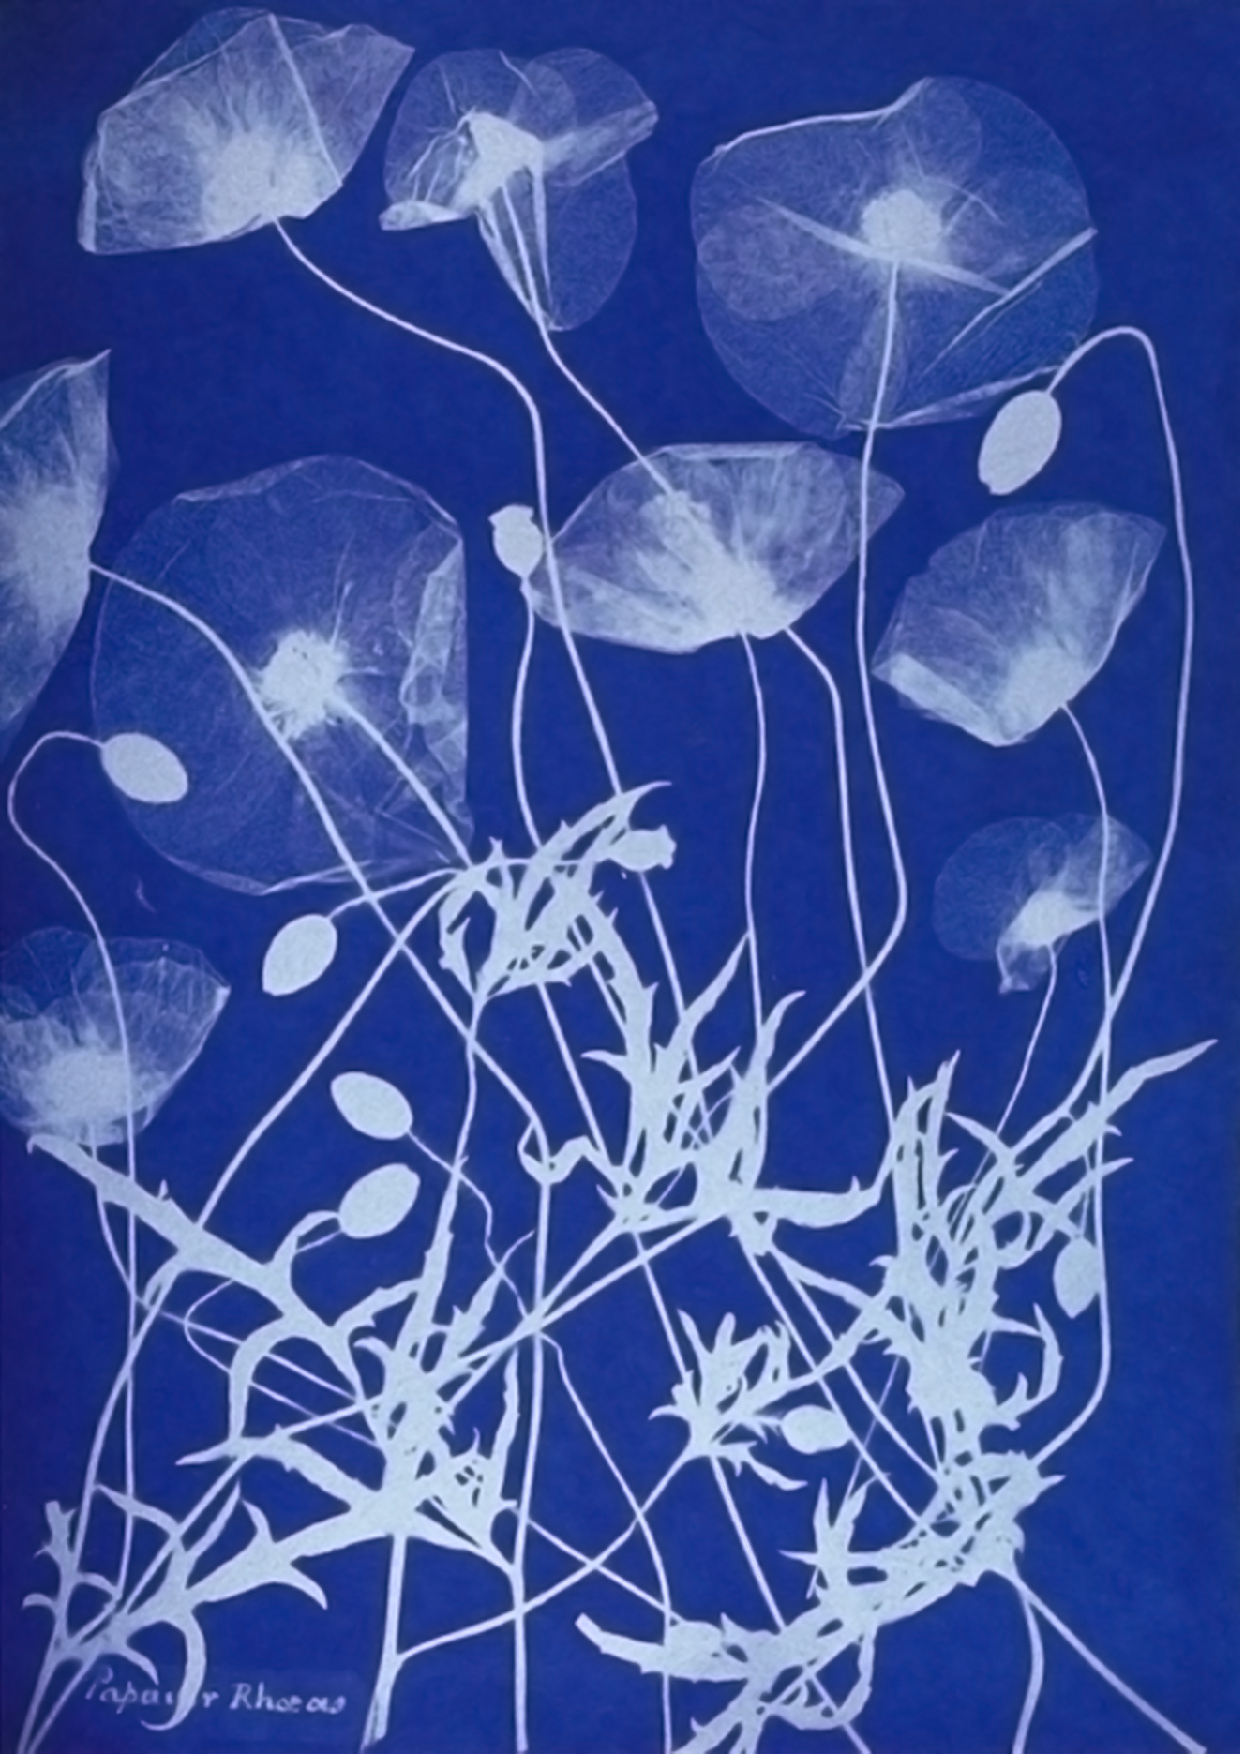
\includepdf{../media/chapter_illustration/papaver_rhoeas}

\chapter{The Poppy development} % (fold)


\section{Introduction} % (fold)

Research in humanoid robotics has been thriving in the recent years~\cite{hirai1998development} \cite{kaneko2008humanoid}, both due to theirs predicted relevance for personal and assistive robotics~\cite{tapus2007socially} \cite{oztop2005human}, and because of the scientific challenges raised by robotics with regards to cognition~\cite{asada2001cognitive}, natural communication~\cite{stiefelhagen2004natural} \cite{breazeal2002robots}, biped locomotion~\cite{yamaguchi1999development} \cite{chestnutt2005footstep} \cite{collins2005bipedal} and full-body physical interaction with the environment~\cite{ude2004programming}.

But like the LHC is an experimental platform allowing to explore quantum mechanics and the origin of our universe,  humanoids can act as simplified and controllable human simulators. Thus humanoid robots can be amazing tools to study human-being and eventually contribute in a better understanding of Human's behaviors and abilities~\cite{atkeson2000using} \cite{cheng2007cb} \cite{brooks1986achieving}.

A famous example of such humanoid uses was the Cog project~\cite{brooks1999cog} at the Humanoid Robotics Group of the Massachusetts Institute of Technology. This research project has two goals: an engineering goal of building a prototype general purpose flexible and dextrous autonomous robot and a scientific goal of understanding human cognition~\cite{brooks1994building}. In particular, this project concentrated on embodiment and interaction intelligence with four aspects of a novel methodology: developmental structure, physical embodiment, integration of multiple sensory and motor systems, and social interaction. For this purpose they build several robotic platform such as a humanoid~\cite{brooks1999cog} (see \figurename~\ref{fig:brooks_and_cog}), and a very expressive multi-articulated head named Kismet~\cite{breazeal2003emotion} (see \figurename~\ref{fig:breazeal_kismet}).

% This project ended in 2003 and has bring great scientific contributions such as ... REF


\begin{figure}[t]
\centering
    \subfloat[][Rodney Brooks and the Cog humanoid]{\label{fig:brooks_and_cog}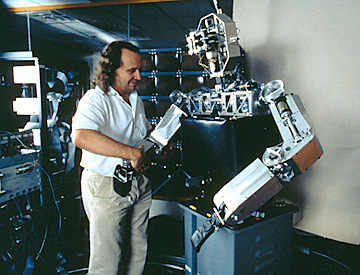
\includegraphics[height=5cm]{brooks_and_cog.jpg}}
    \hfil
    \subfloat[][Cynthia Breazeal with Kismet]{\label{fig:breazeal_kismet}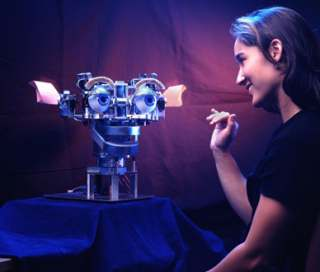
\includegraphics[height=5cm]{breazeal_kismet.jpg}}
    \caption{The Cog project was about the use of computer and robotic technology to better understand and emulate human intelligence.}
    \label{fig:cog_project}
\end{figure}



The context of this PhD thesis is grounded on the same scientific motivations as the work of R.Brooks, R.Pfeifer, T.McGeer and initiative such as the Cog project i.e. exploring the role of morphology, cognition and embodiment intelligence in several aspects using real experimental robotic platforms.

The scientific approach of the Cog robots is oriented toward the exploration of embodiment in several aspects, from the low level mechatronics to head design for social interactions, but robots were built 15 years ago and using classic manufacturing techniques (see \figurename~\ref{fig:cog_project}) that made them expansive, complicated to be modified and especially difficult to diffuse in other laboratories.
We are now in 2014, the makers revolution is in progress~\cite{anderson} and novel technologies allow to rethink the way we design robotic platforms, especially humanoid.

In the previous chapter we presented a methodology to design robotic platform allowing both a free exploration of morphological variations and the diffusion in the research community. This method uses 3D printing to produce mechanical part, Arduino architecture for the electronic system and python-based API for the control.

We think such design methodology can contribute in building better experimental robots while it allows to make the modification of a robot morphology both easy and low cost, and by the use of open source diffusion, it permits the transfer and the reuse of scientific work in other laboratories.
Within this context we have built a whole new humanoid robot called Poppy\texttrademark (see Fig.~\ref{fig:poppy_with_me}).

\begin{figure}[tb]
    \begin{center}
        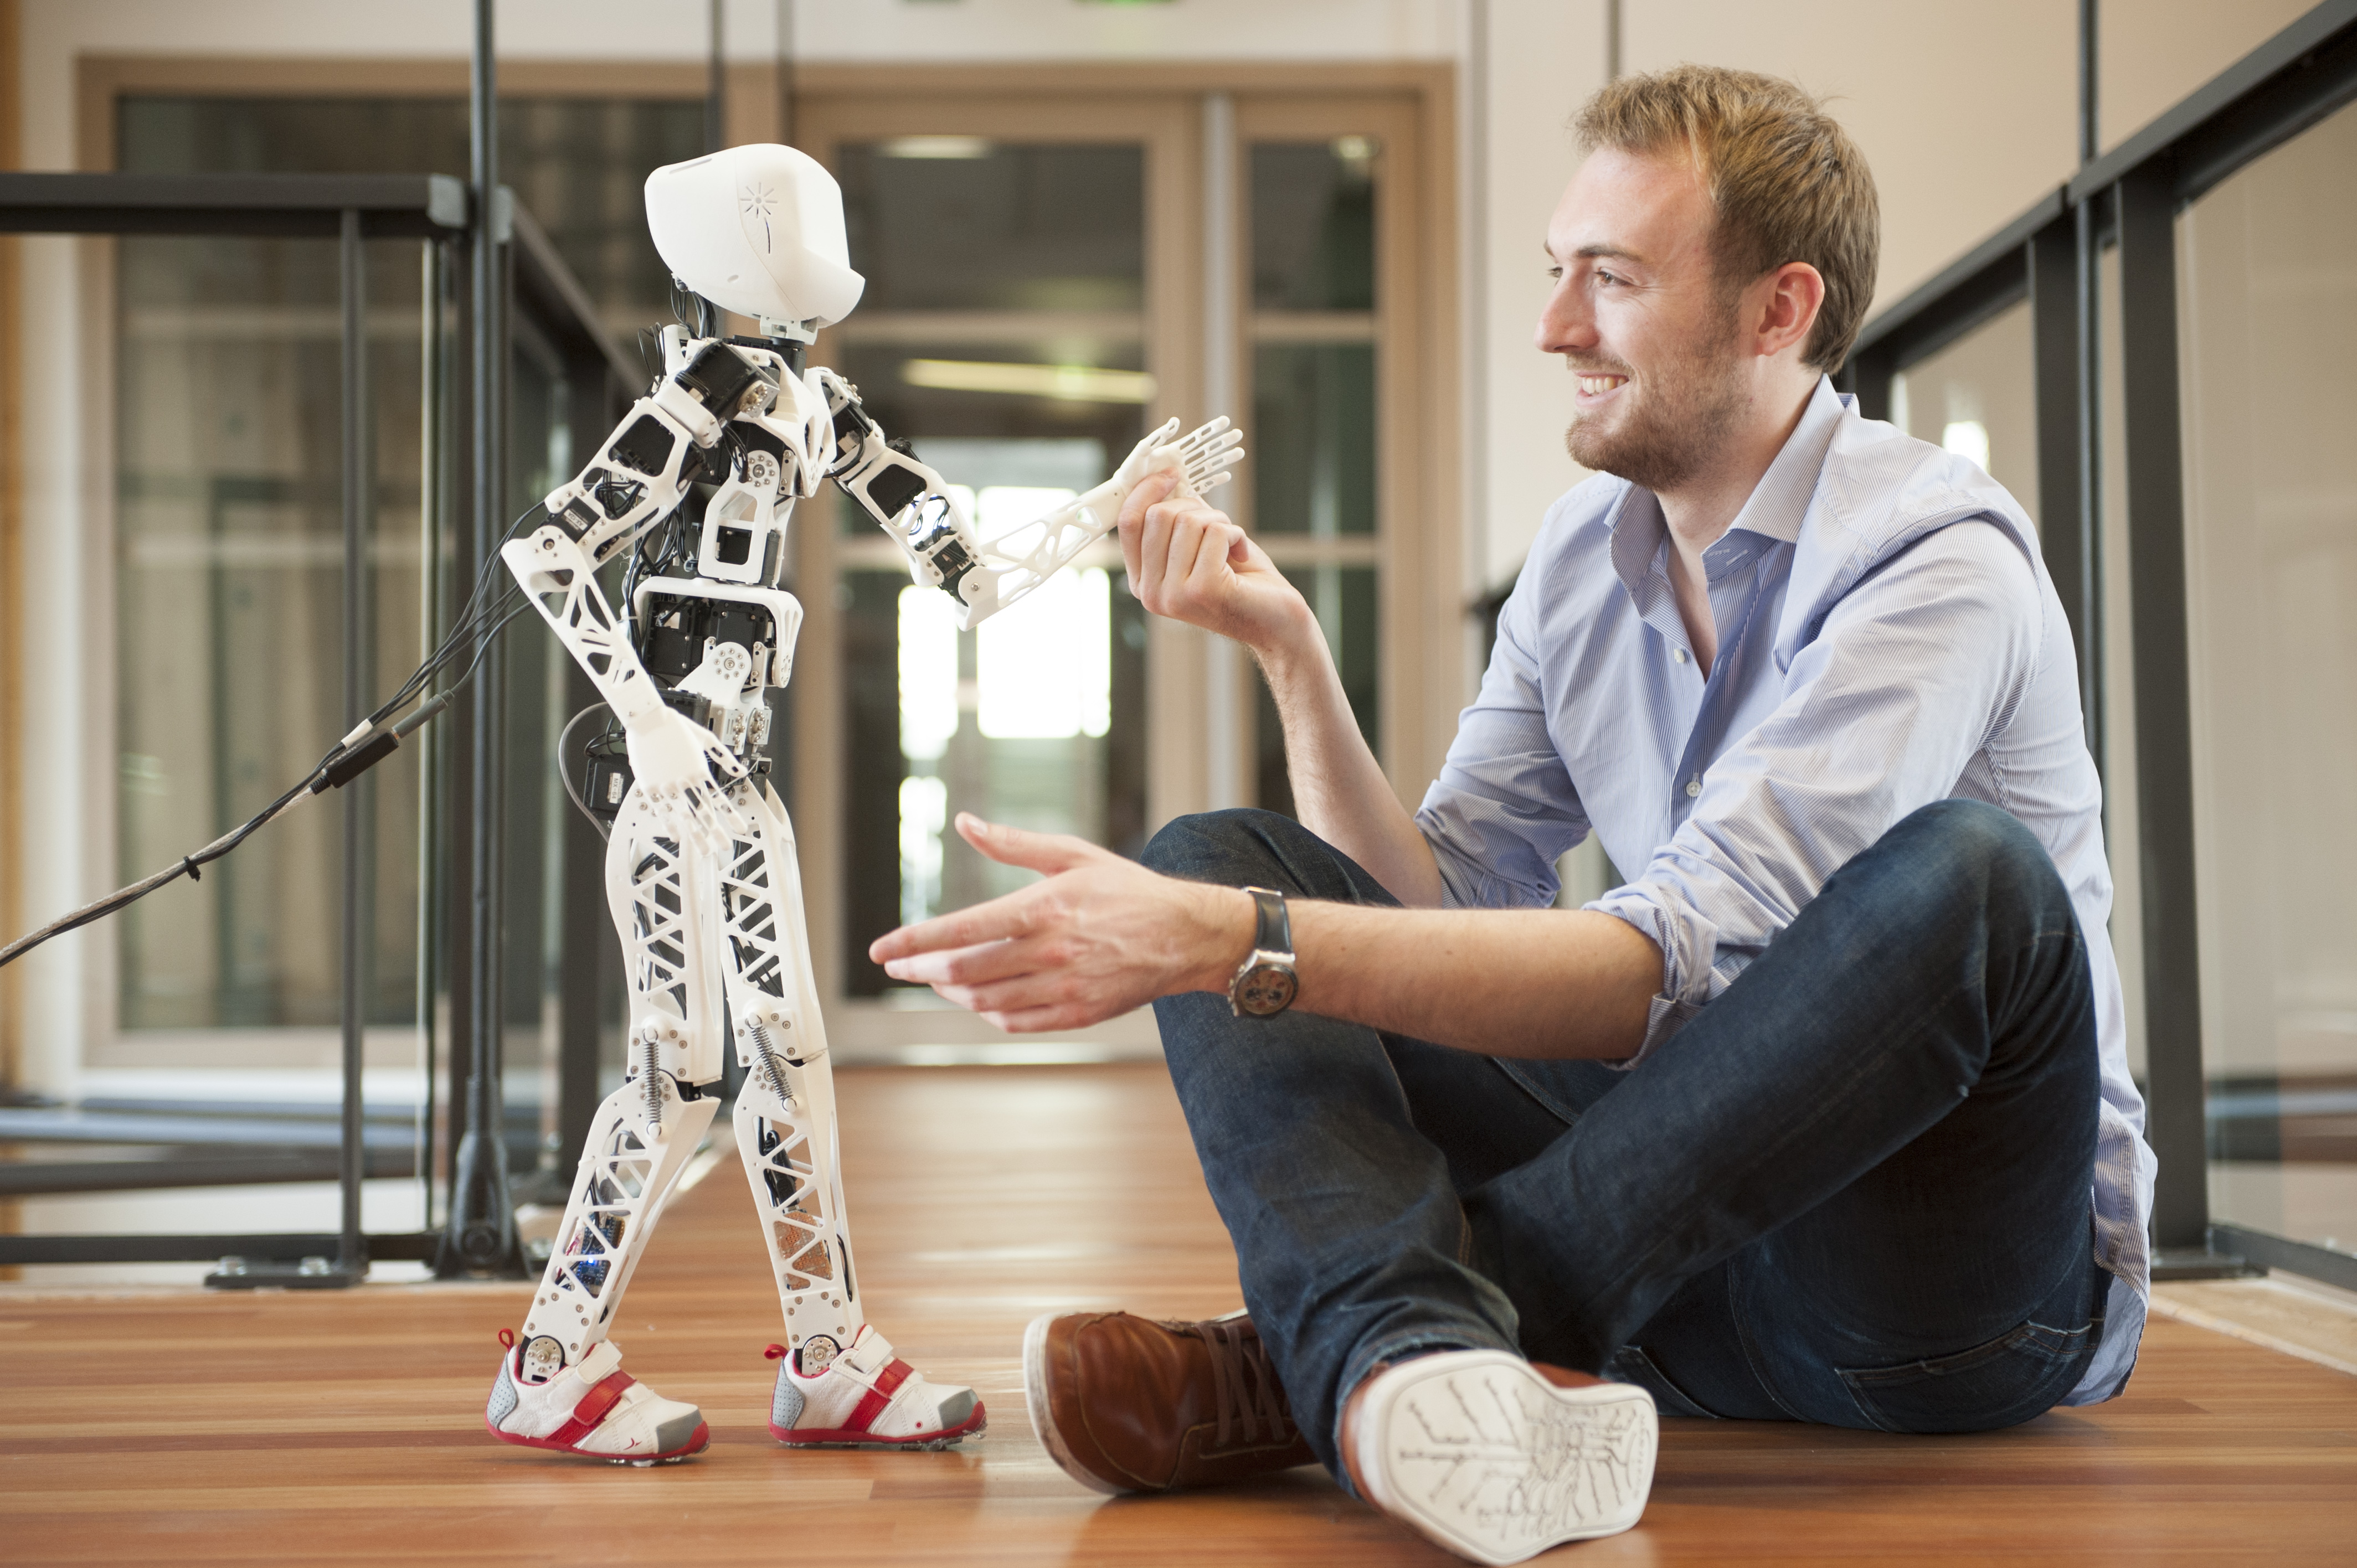
\includegraphics[width=0.7\linewidth]{lapeyre_and_poppy.jpg}
    \end{center}
    \caption{Poppy}
    \label{fig:poppy_with_me}
\end{figure}

This humanoid robot is designed to easily and quickly conduct scientific experiments on sensorimotor learning, exploring morphological properties, and human-robot interaction. As an experimental robotic platform, Poppy is designed to be \textbf{affordable}, \textbf{lightweight}, \textbf{robust and safe}, \textbf{easy to use}, \textbf{highly-hackable} and \textbf{fast and easy to duplicate or modify} with the goal to be easily reproducible and used by other labs thanks to an open source distribution (hardware and software) and the setup of modern online collaborative tools.


In this chapter,  we will describe our motivation, the design guidelines we have followed and the details of Poppy's conception. We will describe with more details the open collaboration associated with the Poppy project in the chapter REF.


\section{Creating a novel humanoid robot} % (fold)

\subsection{Motivations} % (fold)

In 2012, when we started this work, none of the existing humanoid platforms were suitable for exploring the role of morphology. There were two kinds of platform. On one hand the commercial robots, rather easy to use and accessible but with a static and frozen morphology. On the other hand, prototype robots produced in labs to address specific experimentations, studying interesting morphologies but complicated to use and impossible to reproduce outside the lab. In both case, only few are open source, limiting even more hacks, extensions or modifications of their morphologies.

In the Flowers Lab, we had both kind of robot. We used Nao (see \figurename~\ref{fig:nao_platform}) to study human robot interaction (REF PIERRE cadeau). It was really convenient to be use by researchers those are not interested by hardware issue while they are addressing more high-level research challenges. Yet such platform is limited as it is not possible to modify it if the robot is not strictly adapted to our experiment. For example back at this time the Nao camera was not efficient, a closed field of view and a slow framerate. We have difficultly achieved 5 frames/seconds. However, we had the necessary skills to hack Nao and change the camera to fit our needs, but its hardware is not designed to be changed. Improving the vision performance could only be possible by the addition of an external camera on the Nao head which would ruin the user experience. In addition, it would have been interested to explore how the camera parameter (FOV, framerate, resolution,...) can change the user experience but again, it is not possible with such robot.

\begin{figure}[]
\centering
    \subfloat[][Nao]{\label{fig:nao_platform}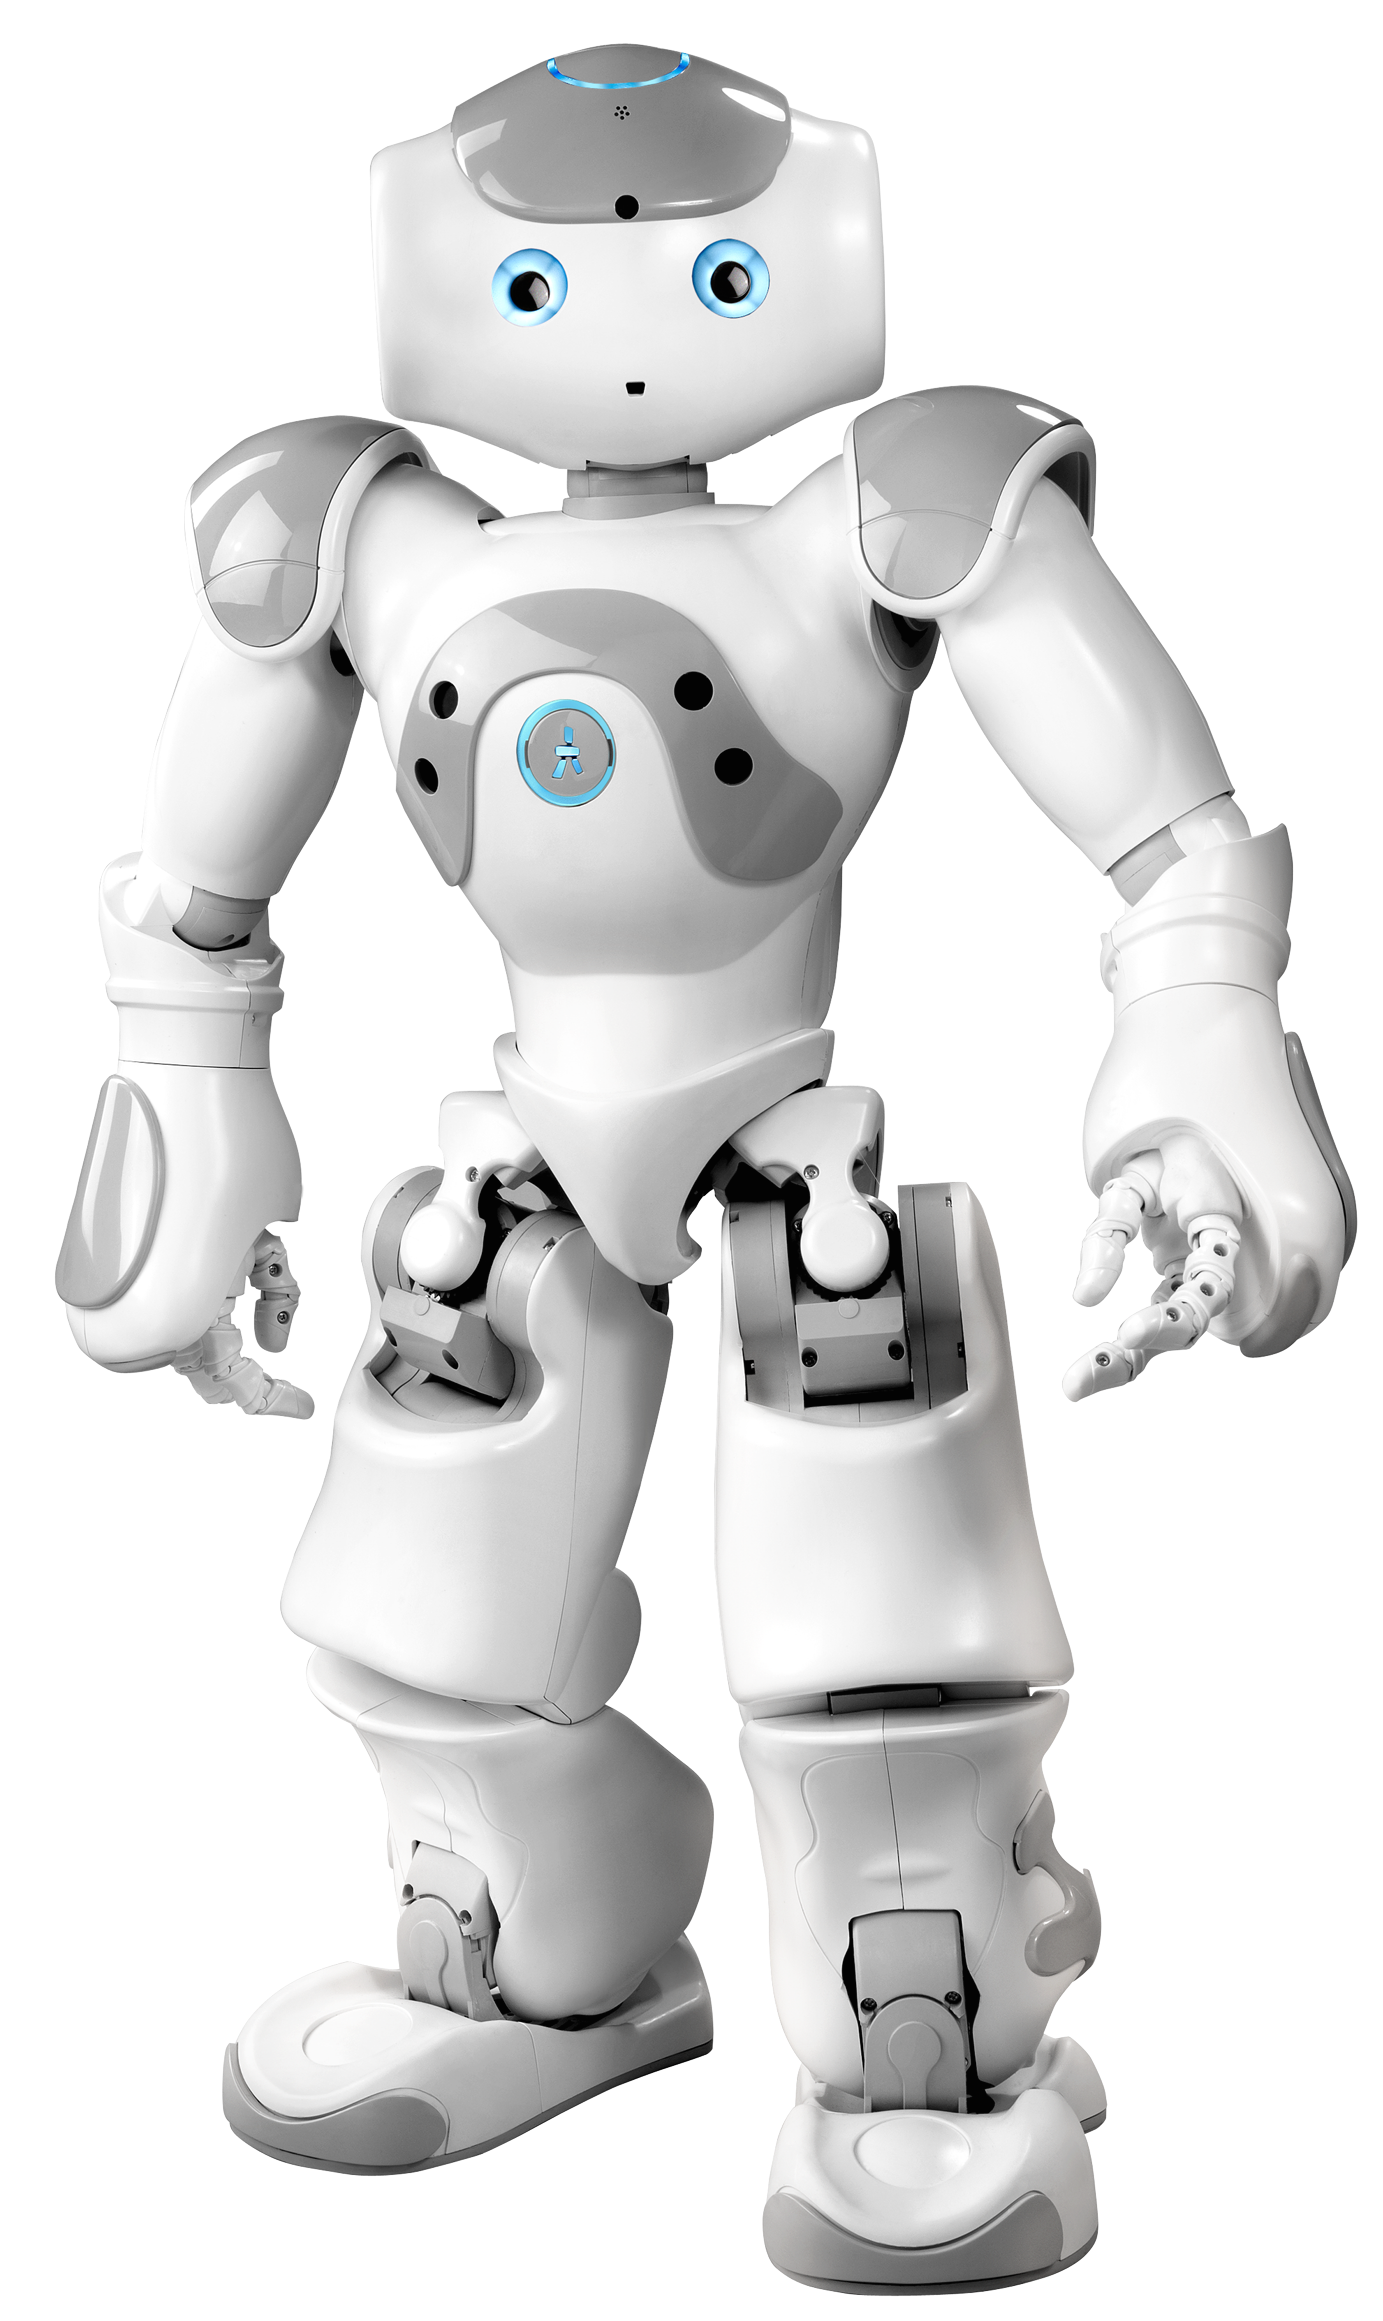
\includegraphics[height=5cm]{nao_face.png}}
    \hfil
    \subfloat[][Darwin-Op]{\label{fig:darwin_platform}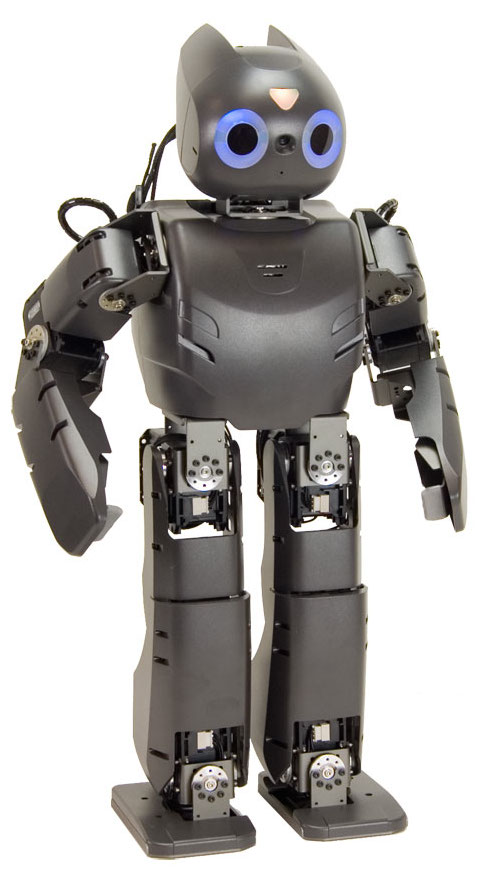
\includegraphics[height=5cm]{darwin_op_face.jpg}}
    \hfil
    \subfloat[][Acroban]{\label{fig:acroban_platform}\includegraphics[height=5cm]{acroban_wout_background.jpg}}
    \caption{None of the existing platform in 2012 was suitable to explore the role of morphology. Nao was impossible to modify. Darwin Op and Acroban used aluminium part really difficult and expensive to produce.}
    \label{fig:2012_Humanoids}
\end{figure}

We also used Acroban (see \figurename~\ref{fig:acroban_platform}) designed by Olivier Ly~\cite{Ly2010}. It is a handcrafted humanoid platform created to explore some morphological properties, especially compliance toward the achievement of dynamic locomotion and playful physical human robot interaction.
While it actually allows modification of its is morphology, its manufacture based on aluminum mechanical parts, Robotis Dynamixel motors, scotch, and rubber bands cobbled together requires lot of effort to be changed. Especially the manufacture of aluminum parts require is complicated and require either very good hand-skills or a 3 axis CNC.
In addition, its use was quite complicated and while several researchers could have been interested by Acroban to study human robot interaction and social acceptance, it was not possible to use it without getting our hands dirty.
Finally, the material and manufacture process make the platform non-stationary. Even if a lab manage to reproduce it, there is a high probability that the physical properties will not be the same. Therefore, the diffusion and the reproducibility of results are limited.


A last alternative would be the use of Darwin Op robot (see \figurename~\ref{fig:darwin_platform}) which is both open source and easily accessible (Robotis sell it already assembled for \$10K), yet as Acroban its hardware based on manufactured metal parts make its morphology very difficult and expensive to be modified (see section REF for more details). Moreover to our knowledge, even if Darwin is open source and very appreciated, its morphology has never be modified by the research community.

Thus one of the main goals was to achieve the design of a humanoid robot which can merge the advantages of both kind of robot, i.e. simple, accessible, reproducible and allowing to easily change and hack its morphology toward custom yet sharable scientific experiments.

\subsection{An experiments-proof robot} % (fold)

Most researchers can attest of the difficulty and frustration raised while conducting robotic experimentation in the real world. We are daily challenged by bugs, technical issues, unpredicted events and side effects. While a bug in a software can be fixed, an error with a hardware platform can cause damages to the robot and postpone the results of an experiment by several weeks.

Therefore many robotic researchers avoid technical issues linked with the real world experimentation by using simple model and physical simulation. But the real world is extremely more complex and rich than the virtual one.
Some high-level behavior experiments are conducted in simulator based on the hypothesis that the real world constraints are not relevant, yet it is really sure ?
Indeed, while the real world constitute a lot of constraints, it is also rich of complex physical effects (gravity, friction, inertia) which should be taken into consideration and could be very useful if interacting with the agent.

As we saw in the related work (chapter~\ref{REF}), the emergence of complex behaviors appear thanks to the interaction between the real world and simple robotic systems. We cannot program behavior because the behavior is the interaction resultant between the program and the real world. Thus we cannot design behavior without the ecological niche of the robot~\cite{Steels1991emergence}.

While using simulator can be helpful as a first step to design robot, it appears incomplete to show results on the role of morphology without real world experimentations.
Therefore, when ones want to study the role of morphology on the robot behavior, being able to explore it in the real world is of paramount importance but unfortunately, current tools make the experimental step really hard to achieve for researchers.

Along our work on building cognitive and developmental learning algorithms, we had experienced these issues, especially while building and using Acroban~\cite{Ly2010} and during the Ergo robot experience (see section~\ref{REF}). Many time has been spent debugging non-robust technologies but it has been very instructive to understand whose are efficient and whose should be avoided.
Therefore Poppy has been designed based on the background experience we have acquired building and using robots acting in the real world. Also to be a really experiments-proof robot, we

\begin{description}
    \item[Robustness and Safety:] Heavy and long real-world experimentations imply a robot should be robust and safe. It should be able to sustain experiments and fall down without easily breaking. At the same time, one should ensure that physical interaction with the robot is safe for humans.
    \item [Precision, stationarity:]Experiments should be repeatable, implying that the robot properties should be stationary.
    \item [Breakable, repairable:] Breaking should not be costly and the robot should be easily repairable.
    \item [Transportable:] To allow for experiments in natural environments, possibly involving interaction with non-technical humans, the robot should be transportable outside the laboratory.
    \item [Easy and fast to duplicate:]Such a reuse of the robotic platform requires that it is easy and fast to duplicate.
    \item [Affordable:]
\end{description}


\subsection{Why being open source is so important ?} % (fold)

Beyond the development of a novel humanoid robot, the open source aspect of the project is fundamental. Indeed, creating a reproducible and sharable robotic platform is one of the main goal of the Poppy project. We want to permit cumulative science with real platform and cumulative science is not possible without a collaborative environment, open source licenses set the official rules of such collaboration.

They are fundamental as people are aware (at least for the main point) of what they can do or not without having to ask to the authors. They are totally free to use the material for their own work and encouraged to do it.

Yet there are also other open source humanoid, Darwin OP and iCub but they use classic manufacturing technique and electronic architecture non-compatible with the exploration of morphology, in addition iCub is very expensive (\$200k) which limit its diffusion as cumulative science tools because few labs have the funding necessary to get one.

Also being open source is not enough, you cannot just drop the files and let people do whatever they want. The creation of a user community is a key to actually transfer open source technology. Indeed, one fundamental aspect of the open source spirit is to create derivative work which can be shared again. The property of the project is transfert to the community when you make it open source.



\section{Poppy overview} % (fold)
\label{sec:poppy_overview}
\begin{figure}[tb]
    \begin{center}
        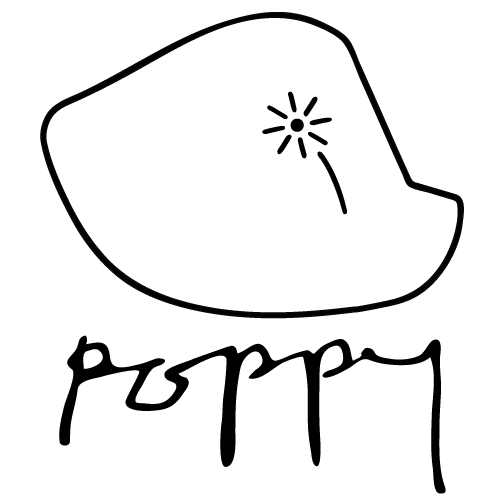
\includegraphics[width=0.5\linewidth]{Poppy_logo_black.png}
    \end{center}
    \caption{Poppy's logo}
    \label{fig:poppy_logo}
\end{figure}

Poppy is the first complete 3D printed open-source and open-hardware humanoid robot (see \figurename~\ref{fig:poppyv0.1_overview}). Its 3D printed skeleton and its Arduino-based electronics are open-hardware (Creative Commons). Its software is open-source (GPL V3), and allows programming beginners as well as advanced roboticists to control the robot in Python thanks to the PyPot library. Its motors are common and widely used off-the-shell Robotis actuators, and allow for compliant control and soft physical human-robot interaction. Poppy presents an original mechanical structure that permits to obtain a light structure with 3.5kg for 84cm height.
Its current morphology takes insight from the human functional morphology: large number of articulation (25 motors), the limbs respect human proportions, it has five articulation in the trunk and its thigh is bended by a $6\deg$ angle similar to the human.

\begin{figure}[tb]
    \begin{center}
        \includegraphics[width=0.95\linewidth]{poppy-overview.pdf}
    \end{center}
    \caption{}
    \label{fig:poppyv0.1_overview}
\end{figure}

Poppy is designed to conduct robotic experiments and integrates several key abilities in an easy-to-use robotic platform toward creating a friendly research framework:


\subsection{Poppy design Guidelines} % (fold)

\subsubsection{Modularity} % (fold)
\label{ssub:modularity}

The whole structure must be easily reconfigurable both for repairing or hacking purposes. This mean the process to replace a Poppy's parts must be simple, low-cost and not require time or special tooling. Also, in order to have a real impact in the open hardware community, special attention is given to the modularity and the reusability of our technological bricks.
Poppy is fully modular (mechanic, electronic, software) allowing to freely explore and modify Poppy's body.
Its modularity and the use of 3D printing make Poppy highly hackable. It can be easily adapted to particular experimental setups.

\subsection{Simplicity} % (fold)
The fact we want to design an easily reproducible robot means we are limited in our design choices. In most case, finding a simple solution avoid the use of an easy solution: we should minimize the number of part and suppliers, be careful of the availability of our parts in each country, take in account the cost and the assembly complexity. All these constraints make the design of the robot way more complex than a unique prototype robot. It also raises some limitation to the main Poppy version while some interesting or efficient solution cannot be kept due to their complexity.


\subsection{Scientific platform} % (fold)

[A lightweight structure and under-actuated:] Many humanoid robots use powerful motors often associated with highly accurate sensors. This has a cost, both in terms of weight and computation resources. Moreover, to ensure the accuracy of the sensory-motor space it is necessary to design very rigid mechanical parts. The whole structure obtained is powerful but very heavy and due to inertia not very agile. This kind of robots can intensively repeat precise and complex movements, but are somewhat uncomfortable when it comes to walking on uneven ground. All mechanical parts were designed to optimize their weight and make the platform Poppy as light as possible. The obtained mass reduction allows the use of less powerful motors which are therefore lighter. We can thus have a lightweight robot, strong and powerful enough to perform tasks such as walking and physical interaction.

[Bio-inspired morphology:] Human being is a great example of biped locomotion ability. Strictly mimicking the human morphology is certainly not a good idea as the element composing a robot are not comparable. However, studying the functional interest of certain human bio-mechanic properties can reveal interesting insight to explore novel humanoid design.

[Ecological balance principle:] The ecological balance principle, introduce by Rolf Pfeifer, states that there is a balance or task distribution between morphology, materials, control, and interaction with the environment. Following this principle, we try to keep a balance between the different part of the robot.

[Whole body compliance:] Important aspects of adaptation to physical obstacles or HRI require humanoid robots to be full-body compliant. This includes both the ability to absorb external shocks due to the passive compliance of the mechanical structure (bendable materials and springs), but also the ability to actively and dynamically control the compliance of motors, which may be either controlled in position with compliance, or directly in torque (thanks to the use of adequate recent servomotor technologies).

Important aspects of adaptation to physical obstacles or to humans require humanoid robots to be full-body compliant. The use of Robotis Dynamixel actuators permits to actively and dynamically control the compliance of motors, which may be either controlled in position with compliance, or directly in torque

\subsubsection{Experimental platform} % (fold)
\textbf{Large sensori-motor space:} Robotis Dynamixel give access to a large number of internal sensors and control parameter. In addition, Poppy has several basic sensors such as IMU, camera and which can be easily extended with novel sensors thanks to the Arduino eletronic architecture.
\textbf{Robustness:} Poppy is designed to be robust to falls and to allow long experimentations (e.g. several hours). Also, its conception, slightly under-actuated, prevents it from destructing itself if wrong moves occur.
    \textbf{Transportable outside the lab:} Its size (84 cm) and weight (3.5 kg) make Poppy an easily tranportable robot. In addition its robustness avoid the installation of complex security system around the platform allowing the use Poppy anywhere.
    \textbf{Easy to setup:} we try to keep Poppy and its modules as Plug’n'Play as possible.
    \textbf{Affordable:} to make Poppy widely accessible, we keep the cost relatively low. You can afford all components for 7500-8000\texteuro or thanks to its modularity, only use the parts of the robot needed.


\subsubsection{Explore interaction} % (fold)
\label{sub:explore_interaction}

\textbf{Social and physical human-robot interaction:} Poppy was designed to afford full-body physical interaction, as well as to afford social interaction, with a head and gestural apparatus that can be programmed for communicative or affective expression.


% subsection experimental_platform (end)

\subsection{Open platform for open science} % (fold)
\label{sub:open_platform_for_open_science}

    \textbf{Easy to duplicate:} the overall time to assemble all mechanic components of Poppy takes about 2 days. Adding extra sensors is simplified by the use of Arduino electronic architecture.
Also we set up several web tools to support collaboration and sharing among members of the Poppy community: a portal web site (\url{www.poppy-project.org}), GitHub repositories for the hardware and software with associated wikis for documentation (\url{www.github.com/poppy-project/}), and a novel generation forum based on Discourse\footnote{\url{www.discourse.org}} technology (\url{forum.poppy-project.org}).
% subsection open_platform_for_open_science (end)



% subsection explore_interaction (end)

\subsection{Take care of the aesthetic} % (fold)
In the scientific community, design and aesthetic are often left aside as a superficial feature. But when an object has to interact with human, the design and aesthetic represent a main communication channels. The interaction with our senses change the way we understand the purpose of a object. As any communication tool, the message we convey can be noised or enforced by the form. Thus the robot appearance must fit the robot abilities and try to give insights to the user about what it can or cannot do.
Both at a macro or micro scale, the Poppy aesthetic is thought to show some conceptual aspects of its design, such as the lightness, the modularity or the fact it is not powerful.
\textbf{A particular design:} Poppy is often complimented for its unique design which draws particular attention.

This is true for the robot itself but also for the whole environment (documentation, video, website).


\section{Highlight of some Poppy's morphological aspects}


\subsection{Bio-inspired body} % (fold)
Toward the design and the exploration of an adapted mechanical structure for biped locomotion, we interested ourselves in how evolution solved sensorimotor tasks related to locomotion and in particular bipedal locomotion. As human locomotion represents one of the finest example of mastering bipedal walking, we took functional inspiration of some elements that seem relevant to improve the locomotion of humanoid robots also the morphological optimization is mainly expressed on the locomotive system (legs and trunks) in order to increase the robot robustness, agility and stability during the walking.

\subsubsection{Human proportion} % (fold)
This bio-inspiration is expressed on the whole structure of Poppy. On the anatomical point of view, it reproduces the human proportions as described in the literature~\cite{dufour2005biomecanique}  (see \figurename~\ref{fig:proportion_poppy}) and their sensorimotor space organization: i.e. the main degrees of freedom (actuated and passive), an inertial unit in the head.

\begin{figure}[]
    \centering
    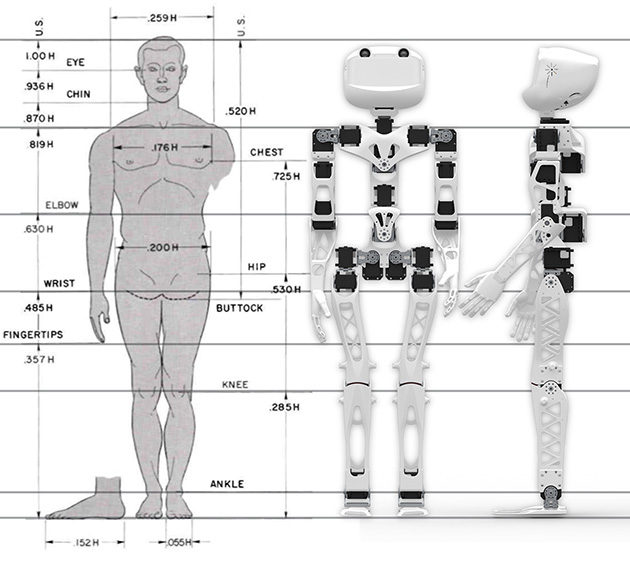
\includegraphics[width=0.9\linewidth]{proportion_poppy.jpg}
    \caption{Human proportion used for the design of Poppy~\cite{dufour2005biomecanique}}
    \label{fig:proportion_poppy}
\end{figure}

\subsubsection{A multi-articulated trunk} % (fold)

Poppy uses the bio-inspired trunk system introduced by Acroban~\cite{ly2010}. Involving five articulations, it allows the reproduction of the main DOFs of the human spine. This feature permits the production of more natural and fluid motions while improving the user experience during physical interaction (see \figurename~\ref{fig:poppy_multi_articulated_trunk}). In addition, the spine plays a fundamental role in bipedal walking and postural balance by actively participating in the balancing of the robot.

\begin{figure}[]
\centering
    \subfloat[][]{\label{fig:frontal_trunk}\includegraphics[width=0.49\linewidth]{trunk_face.png}}
    \hfil
    \subfloat[][]{\label{fig:sagittal_trunk}\includegraphics[width=0.49\linewidth]{trunk_sagittal.png}}
    \caption{Poppy has an articulated trunk of 5 DoFs which allows more natural and fluid motions while improving the user experience during physical interaction and actively participating to the balance of the robot.}
    \label{fig:poppy_multi_articulated_trunk}
\end{figure}

% Contrary to the design of the hips, it was not possible here to fit the 5 motors in the frontal plane due to the limited space in the trunk. So to reduce the shifting of the center of gravity to the back of the robot we gradually shifted the upper body to the front. By doing so, we keep the CoG in the support polygon.

\subsubsection{The bio-inspired thigh} % (fold)
The shape of the thigh is inspired of the human thigh. It is bended by angle of 6\textsuperscript{o}, increasing the stability of the robot during biped locomotion. In the chapter~\ref{REF} we will compare this design with a more traditional straight thigh. We will describe both the theoretical model and real experiments showing that the bio-inspired thigh allows the reduction of falling speed by almost 60\% (single support phase) and the decrease of the lateral motion needed for the mass transfer from one foot to the other by 30\% (double support phase) while reducing the upper body perturbation by about 45\% indicating a more stable walk.

\subsubsection{Foot design} % (fold)

To allow efficient and human-like walking gait, Poppy's feet design takes some functional inspiration from the actual human foot such as the proportion, compliance and toes which are key features concerning both the human walking and biped robots with a human-like gait. In addition, we wanted to reduce the weight (i.e. reducing inertia) of the feet to increase the robot agility. To keep the foot as light as possible while conserving functional properties we decided to use a single motor for the main motion (sagittal plane) while other DoF are passives.

The lateral motion of the foot is limited: few range of motion, low torque. The need of a 360 deg and high torque motor seems over rated. Technically the addition of a motor lead to a major weight gain. We preferred to design  instead a passive joint using torsion spring.

\textbf{Author's note:} A new feet is currently under development and will be released in the incoming weeks. This part will be updated.

\subsection{Lightweight and compliant structure} % (fold)
Following ecological principles~\cite{pfeifer2005new} we decided to design a lightweight and compliant robot requiring low actuation power. All our design choices, such as the materials, the motors or the sensors, have been made to have a balanced morphology.




\subsection{Social and emotional skills} % (fold)

In our lab we are especially interested by the role of morphology for dynamic task such as biped locomotion or physical human robot interaction. Yet Poppy is designed to be a multipurpose robot adapted for several kind of scientific exploration.
An important and challenging research topic is the natural human-robot communication so we have provided Poppy with some basic features allowing to directly explore social human-robot interaction and thus extend the potential research community users.

\subsubsection{Expressive head} % (fold)
Strong technical constraints was imposed because the head embed most of electronic components of Poppy plus a wide 4.5" screen and cameras for social communication. Therefore lot of effort have been invested in the design and aesthetic of Poppy's head (see \figurename~\ref{fig:poppy_beta_head}), both its identity and main communication apparatus. It takes inspiration in robotics, animals, object design and art (see the associated pinterest board \url{http://www.pinterest.com/matthieulapeyre/robot/}). We tried to make it cute, expressive and simple.

\begin{figure}[]
\centering
    \subfloat[][The first assembly]{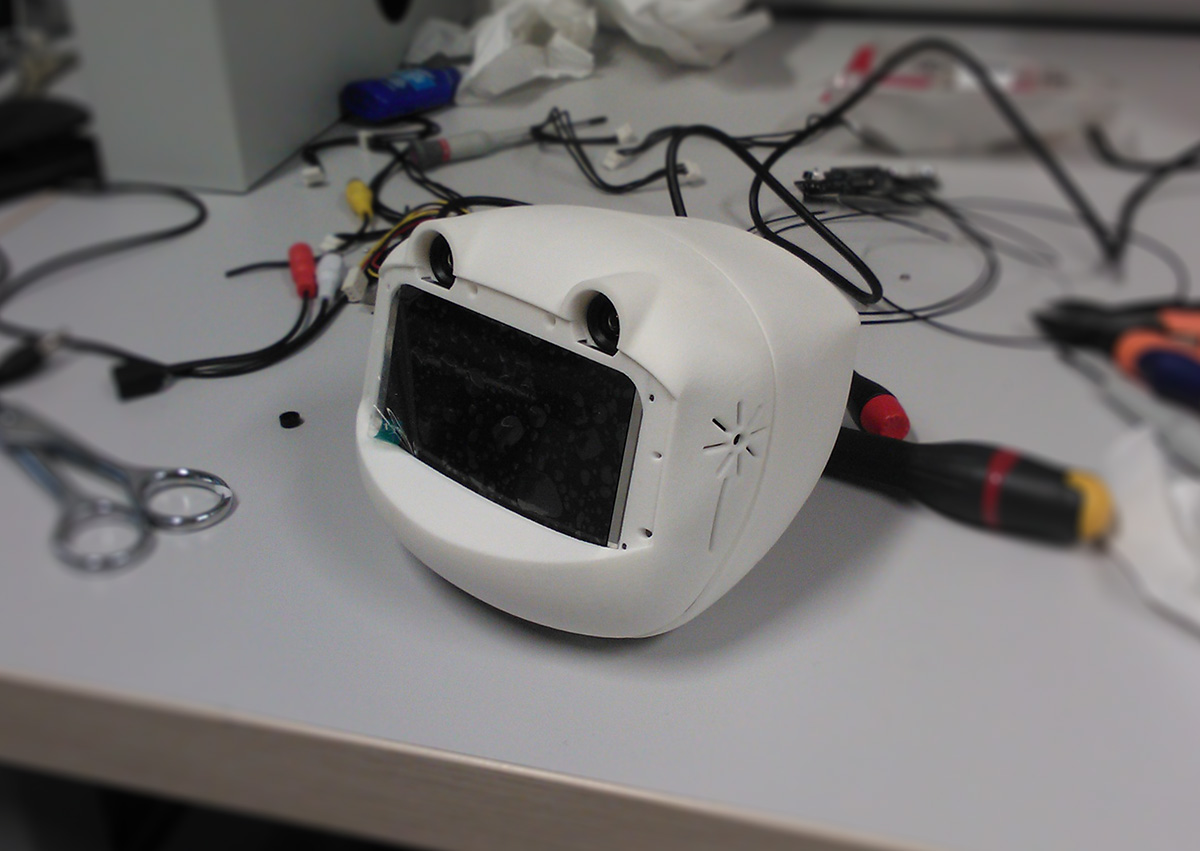
\includegraphics[height=5cm]{head_beta_assembled.jpg}}
    \hfil
    \subfloat[][Screen powered on with basic eyes display]{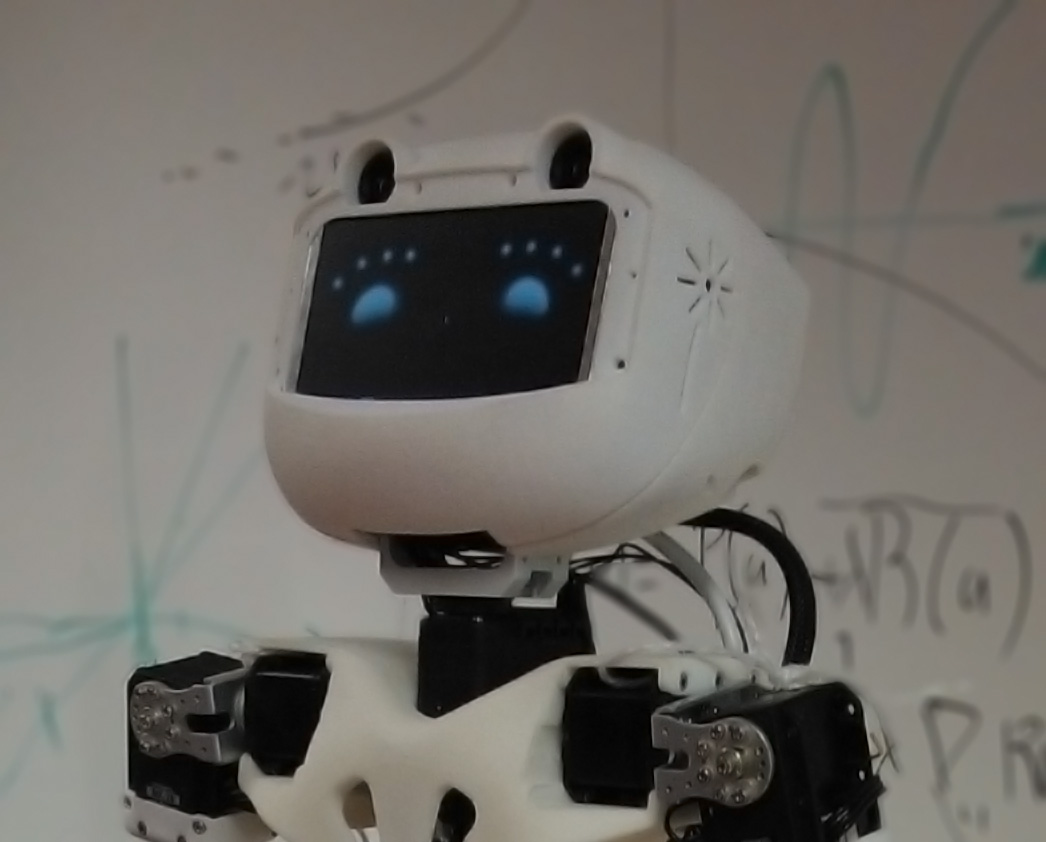
\includegraphics[height=5cm]{poppy_beta_eyes.jpg}}
    \caption{}
    \label{fig:poppy_beta_head}
\end{figure}

However, in the first version showed here, there is a major design error. Indeed my desire was to have a screen to create and explore freely expressive eyes but the use of two visible cameras changed the way people saw Poppy's head. Of course, people seeing 2 cameras considers they are the eyes of the robot and therefore extrapolate that the screen may be the mouth.

We are working on this issue by replacing the two big camera by a small one with a pinhole lens which can be hidden on the Poppy face.


\subsubsection{Compliant and multi-articulated body} % (fold)

Thanks to its multi-articulated structure and its expressive head, Poppy has a particularly high potential for creating and studying emotions and gesture social communication (see \figurename~\ref{fig:TER_cognitic}).

\begin{figure}[]
\centering
    \subfloat[][\url{http://youtu.be/StFIMuyz11M}]{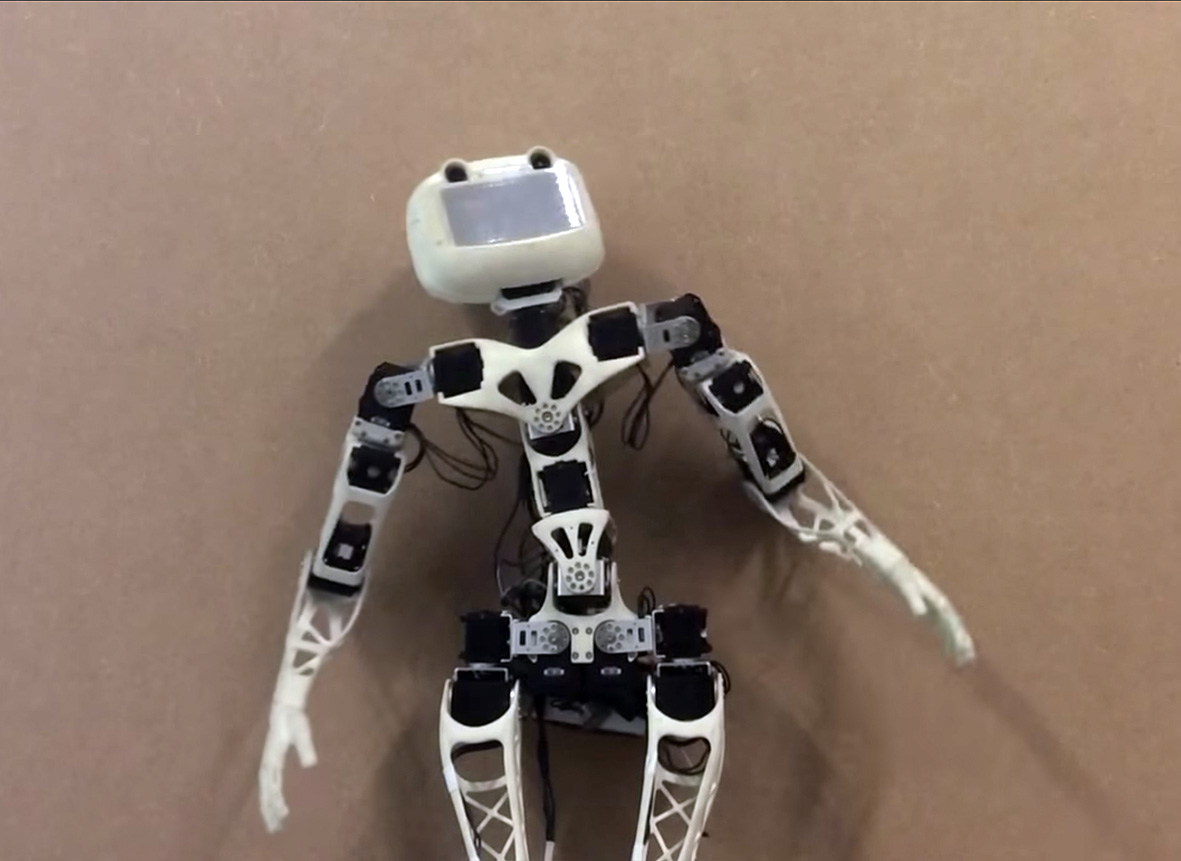
\includegraphics[width=0.45\linewidth]{TER_surprise.jpg}}
    \hfil
    \subfloat[][\url{http://youtu.be/RwCtNwLk10E}]{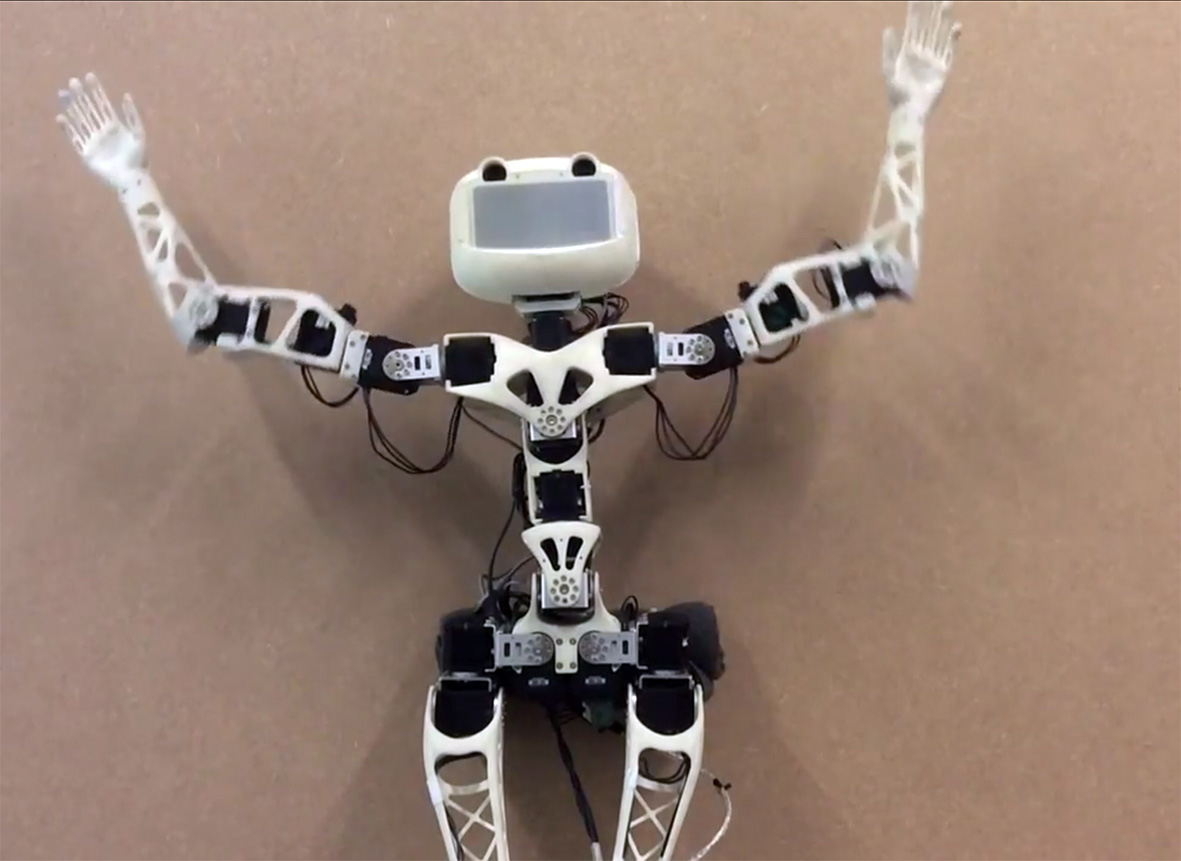
\includegraphics[width=0.45\linewidth]{TER_joy.jpg}}\\
    \subfloat[][\url{http://youtu.be/qrcmLXbpUVo}]{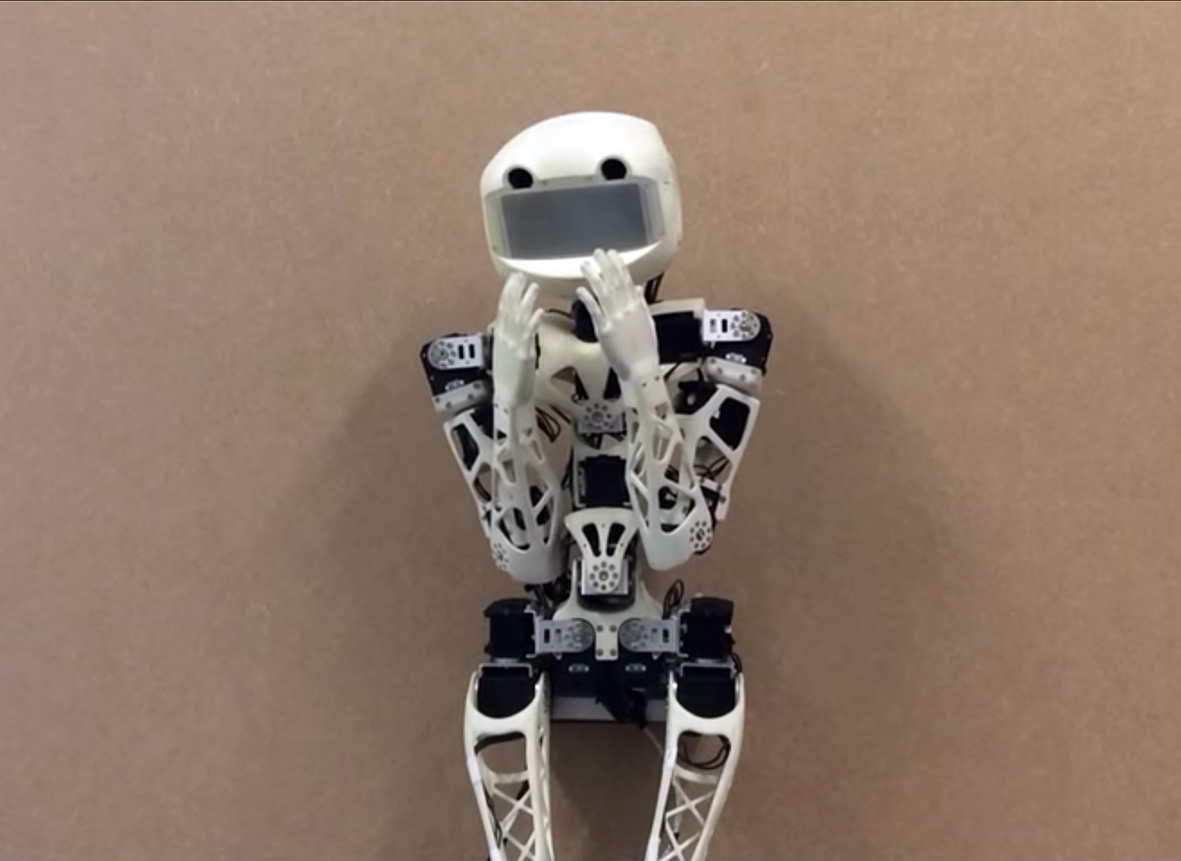
\includegraphics[width=0.45\linewidth]{TER_sad.jpg}}
    \hfil
    \subfloat[][\url{http://youtu.be/ms2niFLevv8}]{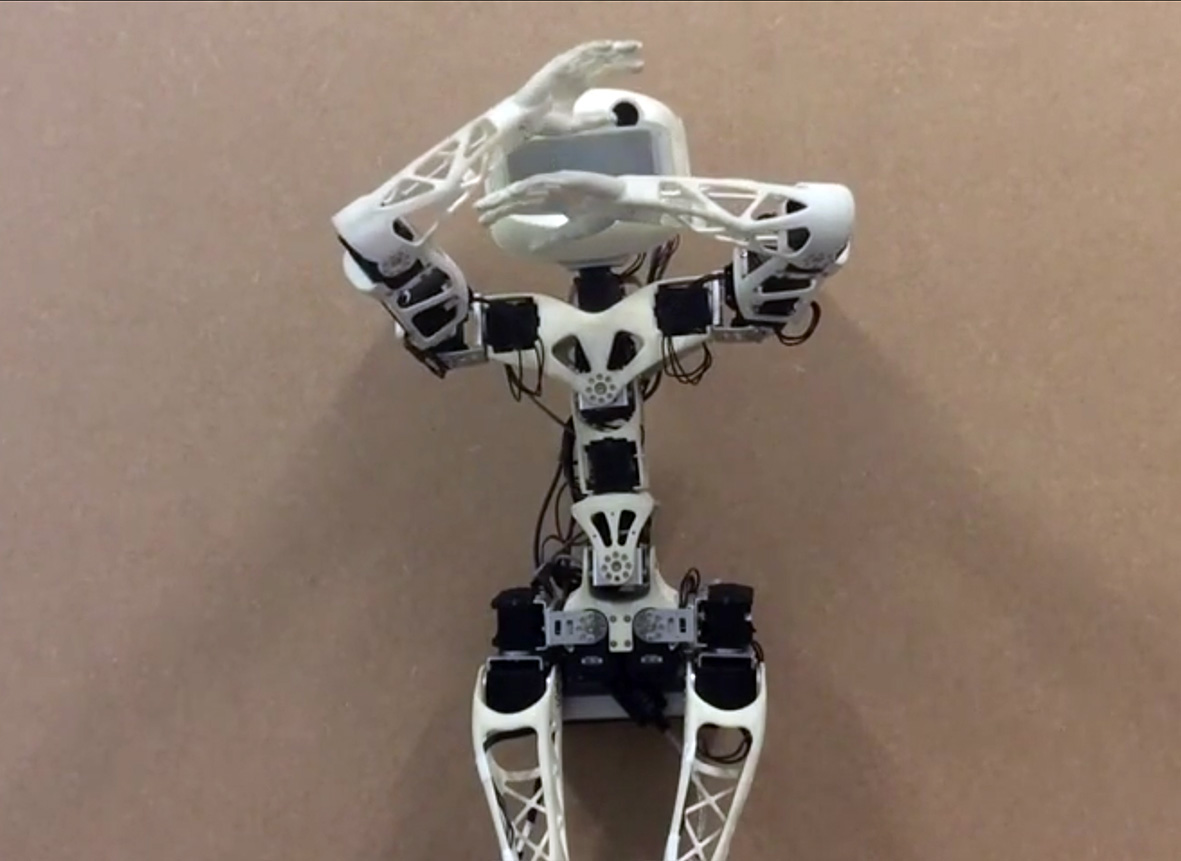
\includegraphics[width=0.45\linewidth]{TER_fear.jpg}}
    \caption{}
    \label{fig:TER_cognitic}
\end{figure}



\section{Design of Poppy's head} % (fold)

\begin{figure}[tb]
    \begin{center}
        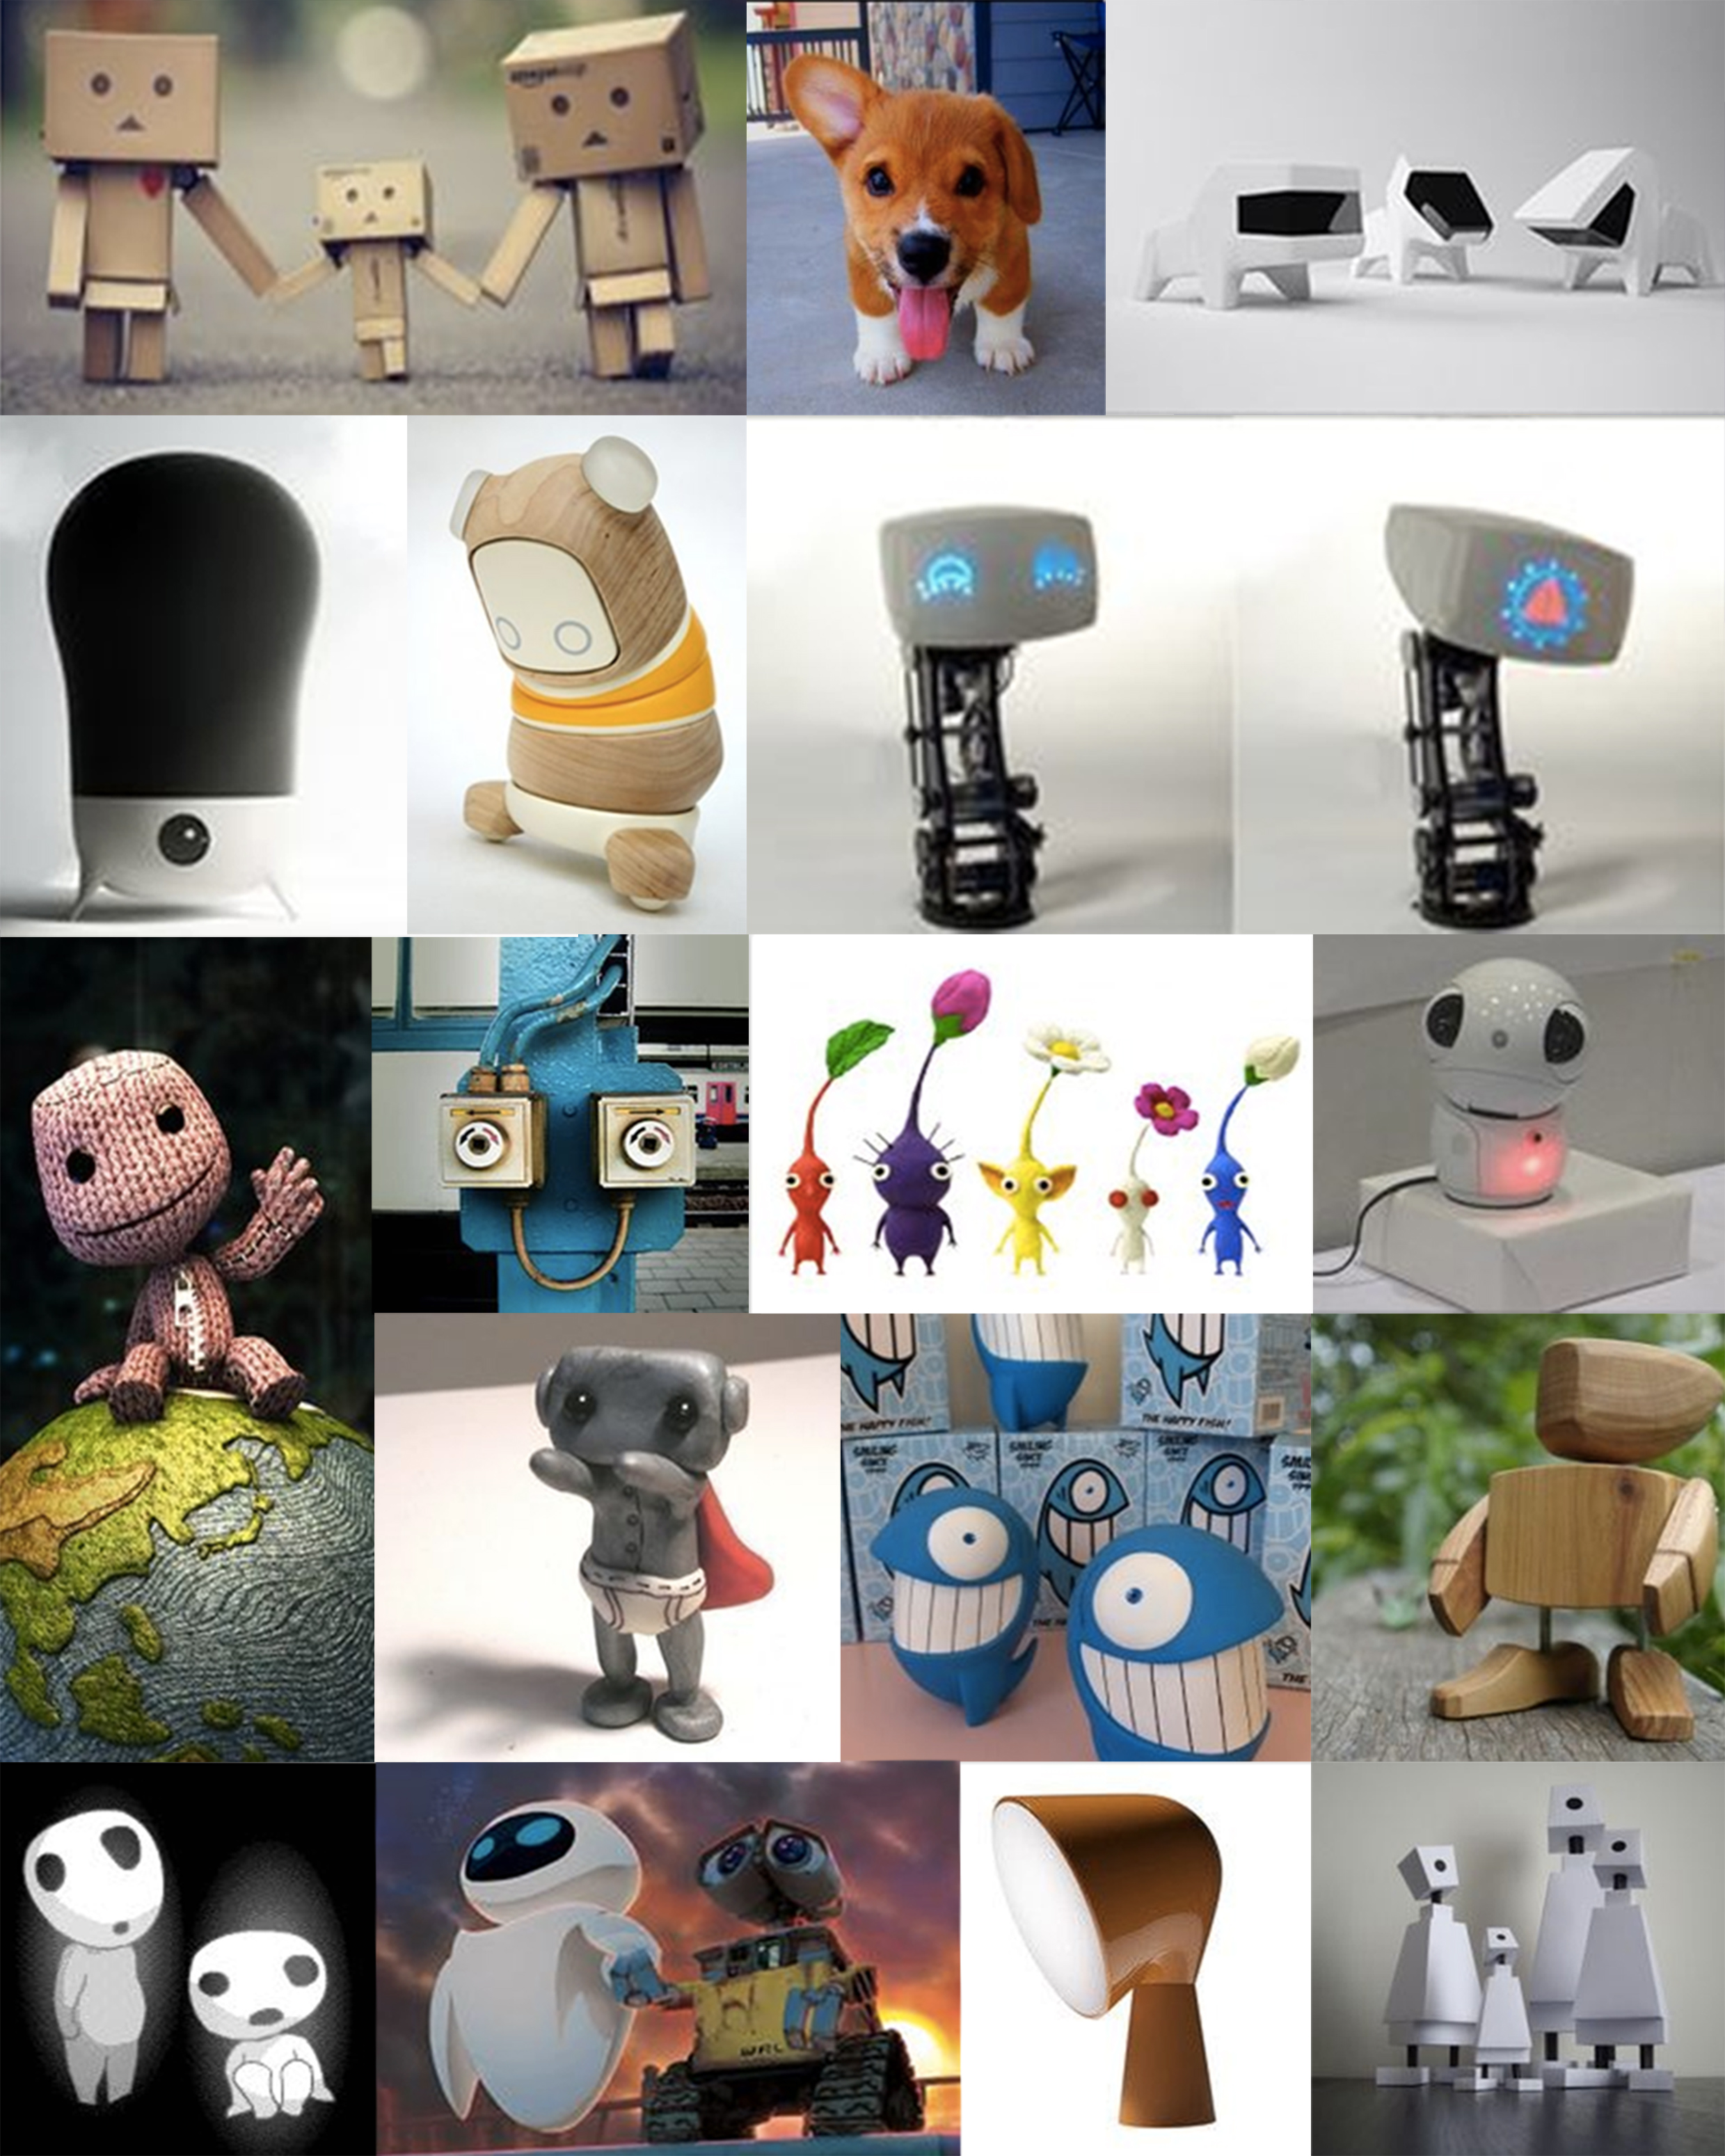
\includegraphics[width=0.8\linewidth]{head_inspiration.jpg}
    \end{center}
    \caption{Caption here}
    \label{fig:figure1}
\end{figure}

\begin{figure}[tb]
\centering
    \subfloat[][]{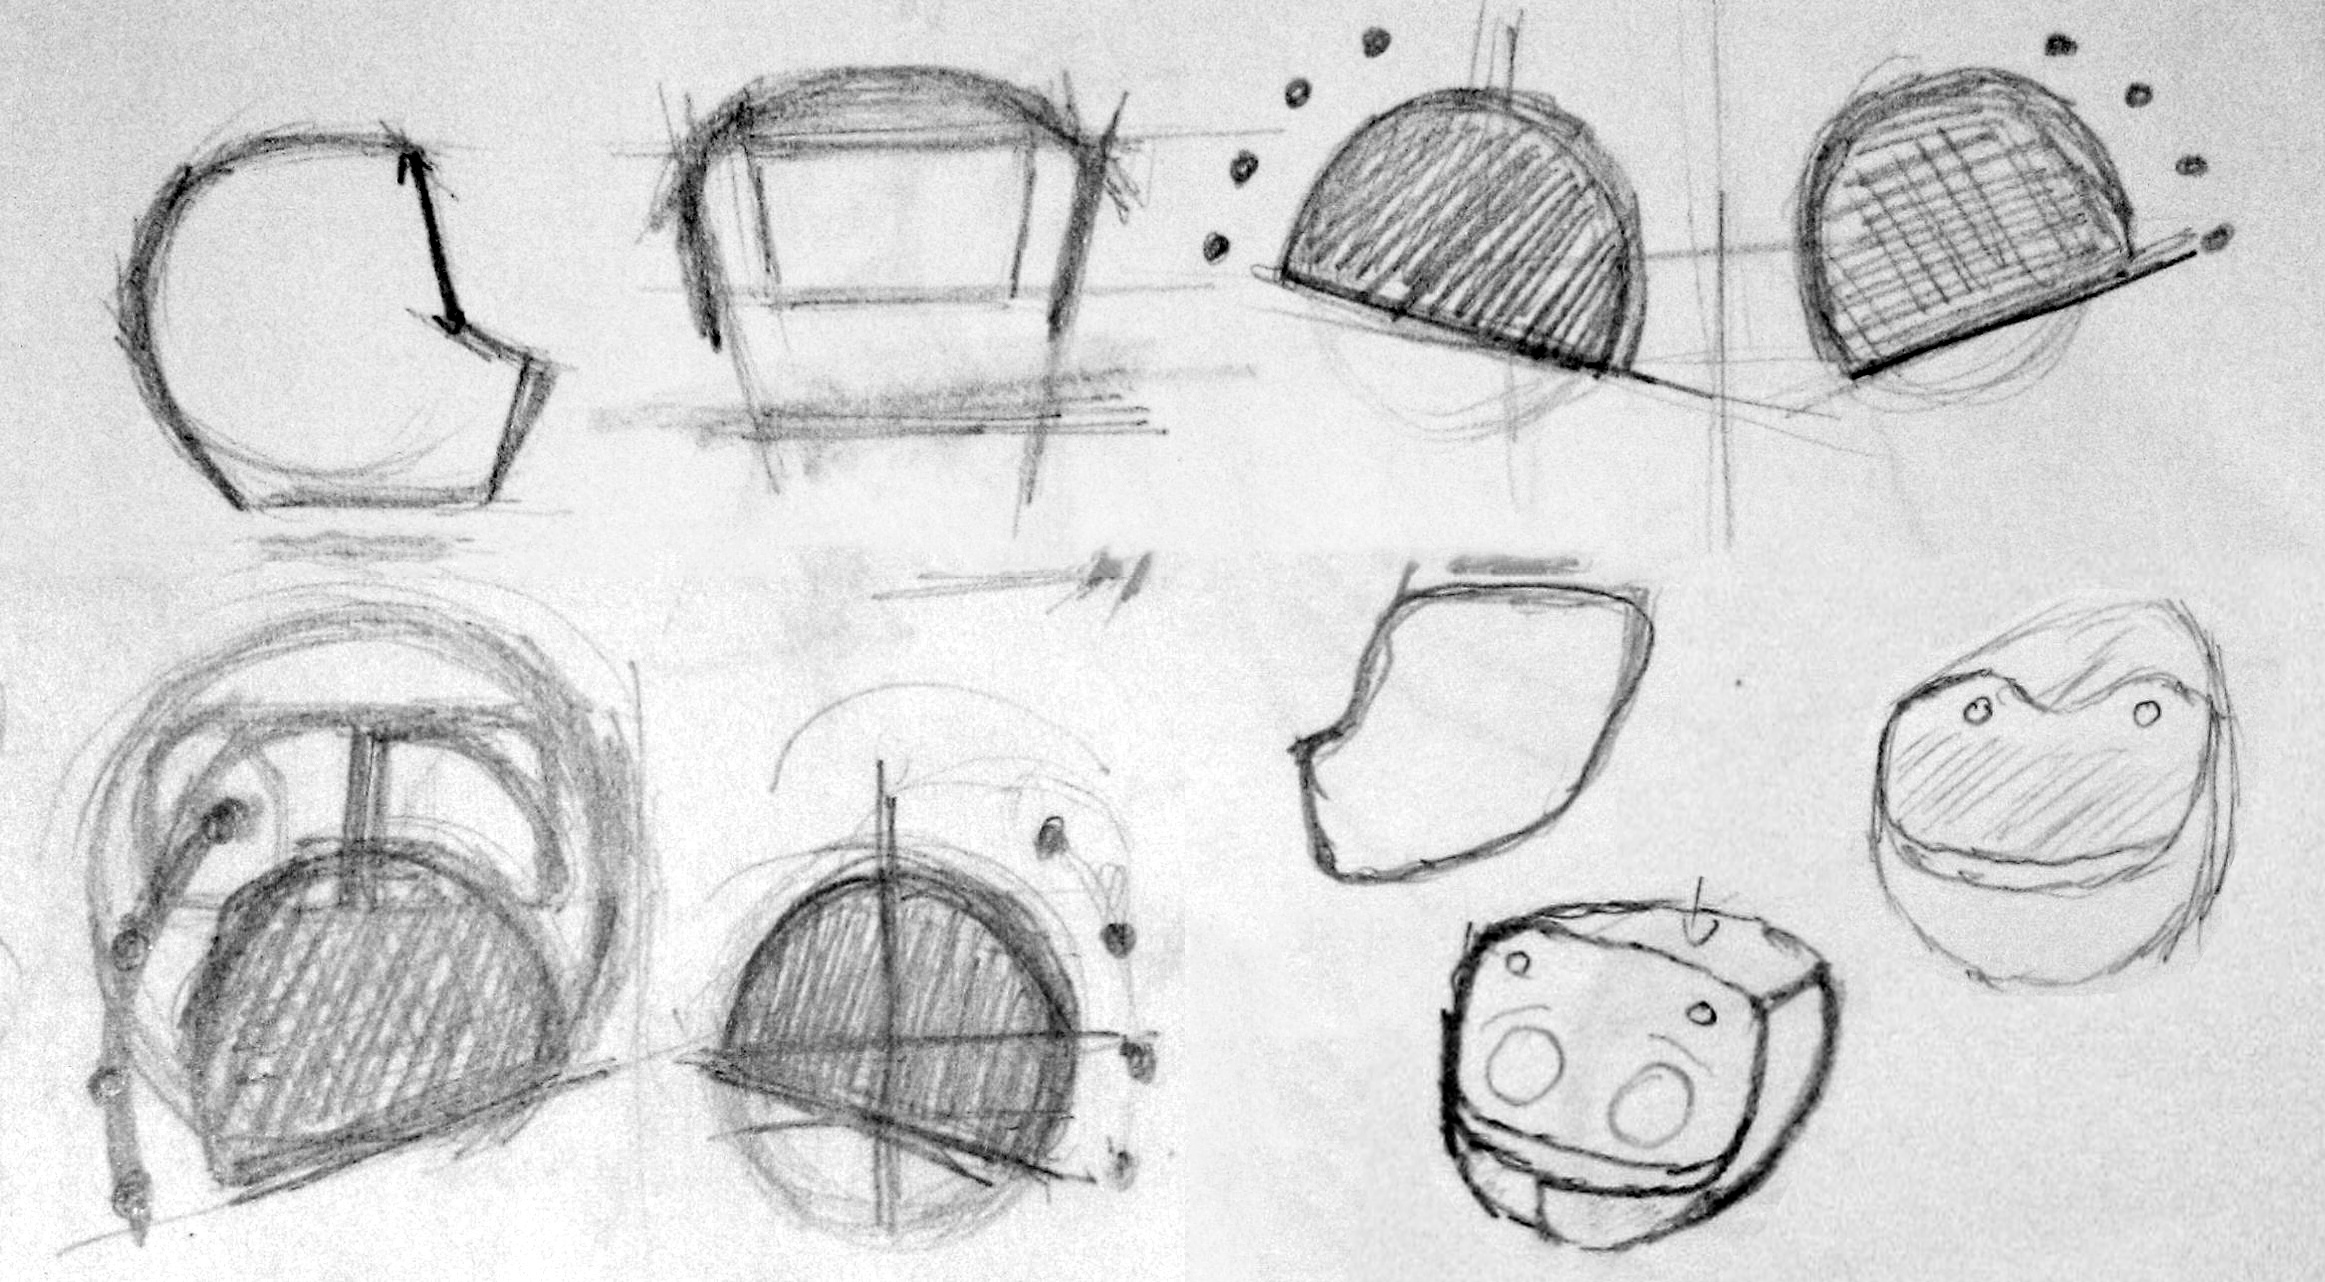
\includegraphics[width=0.48\linewidth]{first_sketch.jpg}}
    \hfil
    \subfloat[][]{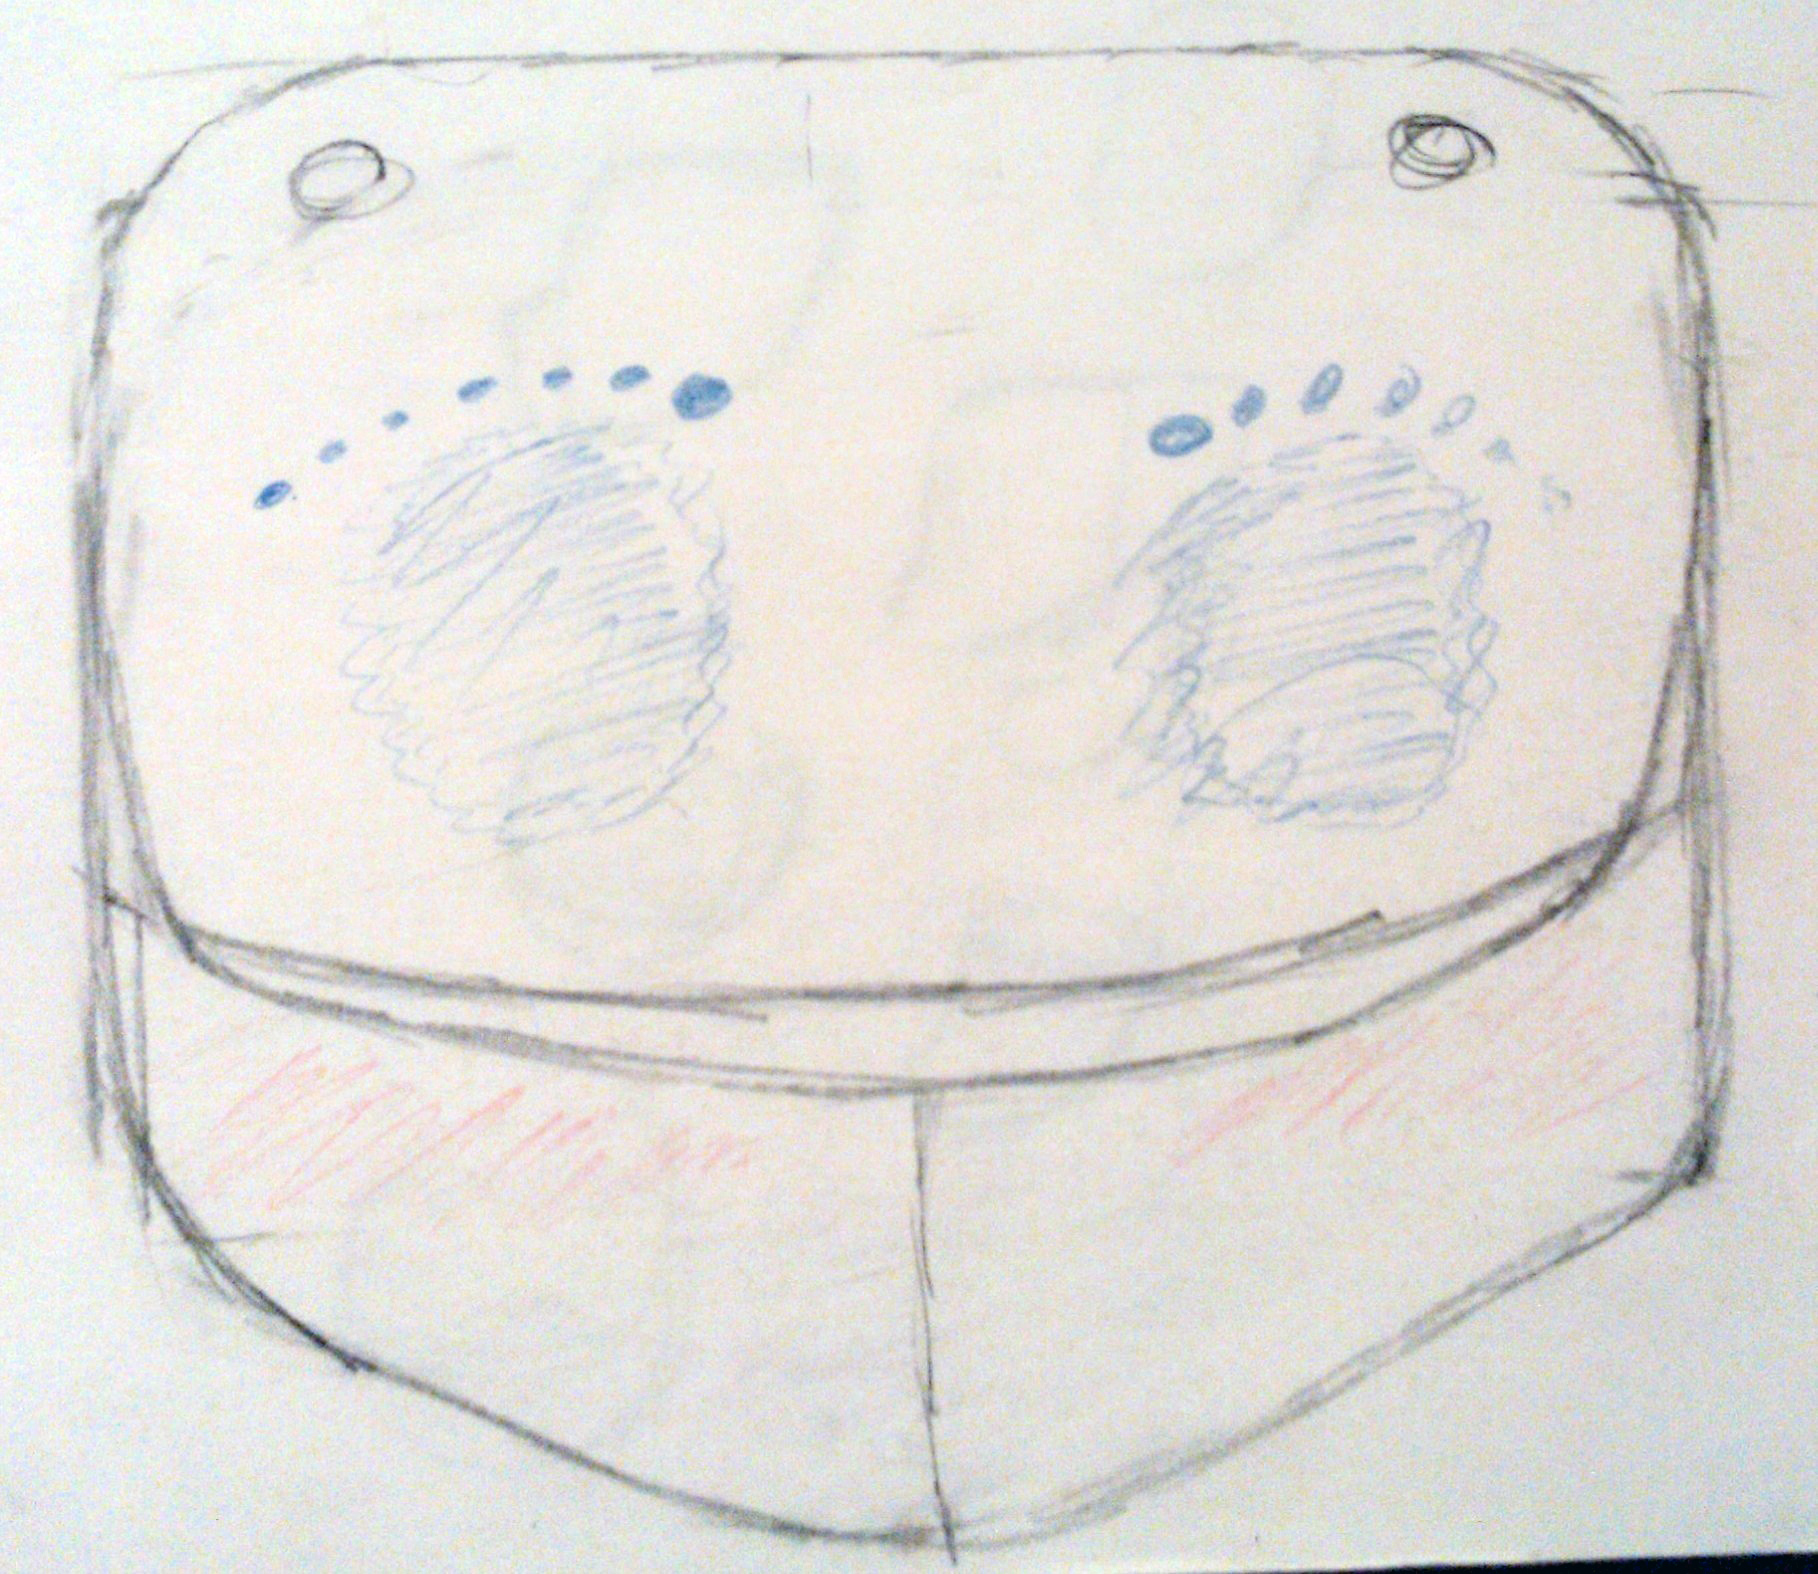
\includegraphics[width=0.48\linewidth]{poppy_head_sketch.jpg}}
    \caption{First hand sketch}
    \label{fig:head_sketch}
\end{figure}


\begin{figure}[tb]
    \begin{center}
        \includegraphics[width=0.8\linewidth]{comparaison_head_betaVs1.jpg}
    \end{center}
    \caption{Caption here}
    \label{fig:figure1}
\end{figure}


\begin{figure}[tb]
\centering
    \subfloat[][]{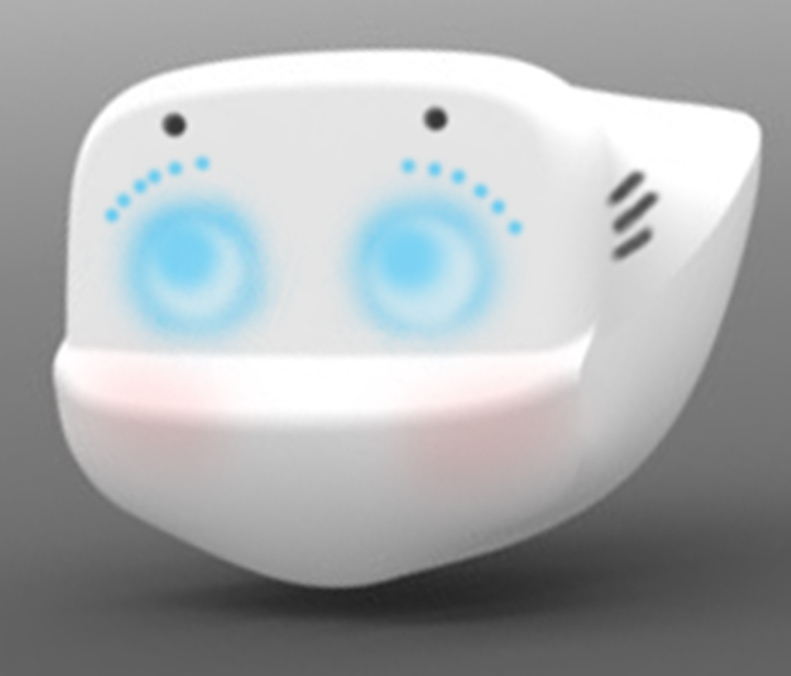
\includegraphics[height=4cm]{head_first_trial.jpg}}
    \hfil
    \subfloat[][]{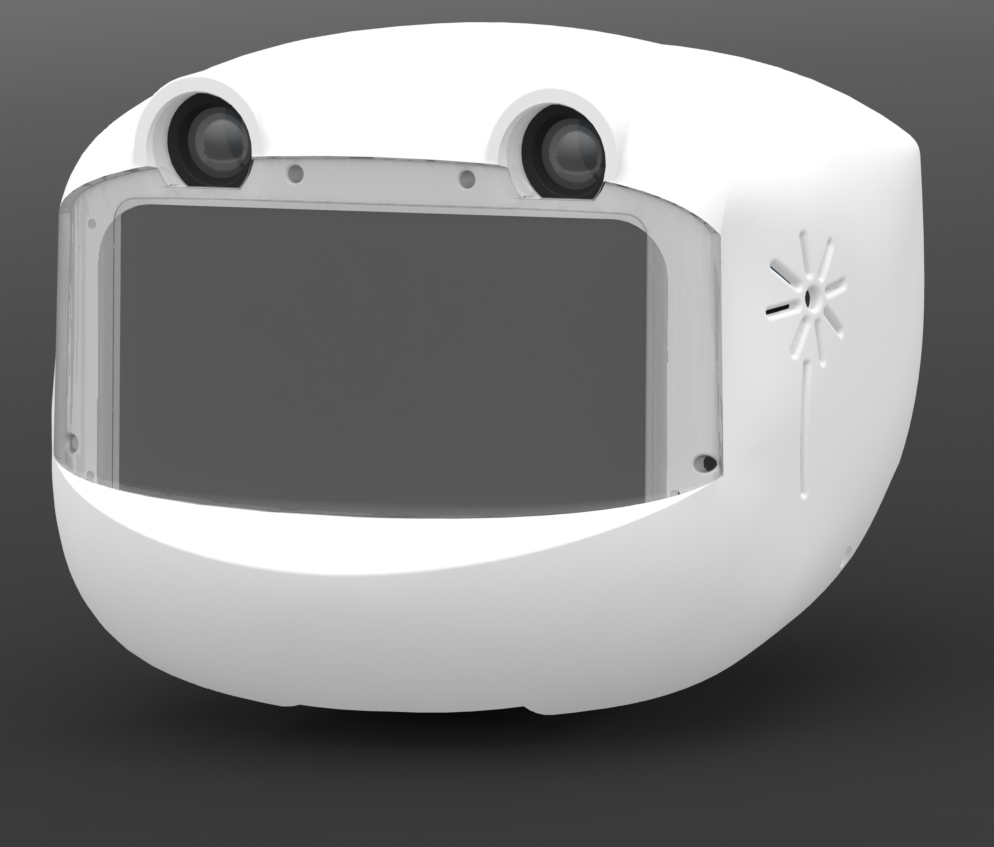
\includegraphics[height=4cm]{head_beta.jpg}}
    \hfil
    \subfloat[][]{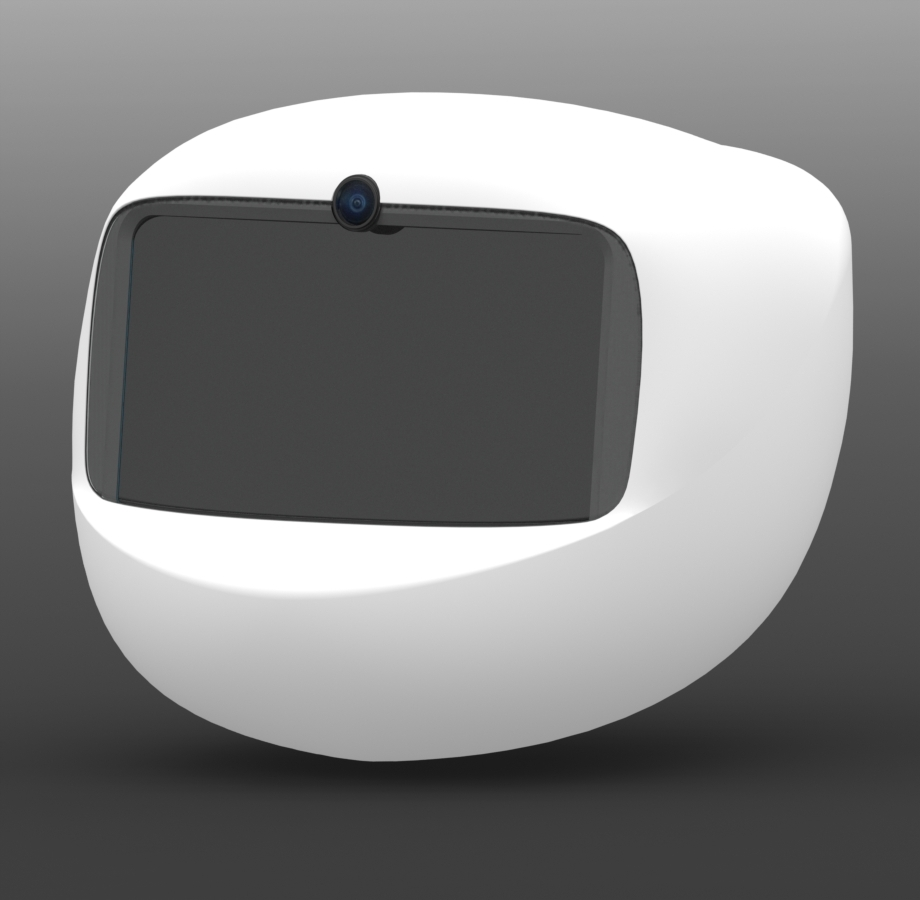
\includegraphics[height=4cm]{poppy_v1_head.jpg}}
    \caption{Evolution of the design}
    \label{fig:head_evolution}
\end{figure}


% section design_of_poppy_s_head (end)


\section{The electronic architecture} % (fold)

The first instance of Poppy (beta version) had a handmade electronic which required hacking several components before soldering them together. This design was not compliant with the design guidelines of Poppy and was actually the main reason Poppy was considered as a beta version. Recent work has been done toward the simplification and the reproducibility of the electronics part.


To keep the spirit of the project described by its guidelines (see previous section REF), the electronic architecture has to be simple, easily repoducible, relatively low-cost and modular. Of course the performance of each components is very important and should be coherent with the ecological balance principle which state it should have a balance between the capacity of each element in the body. For instance, while the robot is not moving fast having a 120 fps 5Mpx camera is an over-kill which can have consequences on the whole electronic architecture.

Yet the electronic integration is challenging. Indeed, because Poppy has 5 degrees of freedom in the torso, there is not enough room for all electronic components needed. Therefore we had to embed most of them in the head which raise a room problem but also a mass problem.

The modularity of the electronic allows to consider the sensory-motor space as an experimental variable (see chapter REF). Being able to change it easily is a paramount importance in the Poppy project and we decided to use Arduino ecosystem for this purpose.

Arduino has developed both hardware and software allowing to create and program electronic system very easily. Their boards have plenty of I/O pins (digital and analog) suitable to connect and control almost anything which is powered by moving electron. The software they developed abstract all the complexity and you can turn a led on or off plugged on one of Arduino board I/O pin with just one line of code.

In addition, Arduino has an growing community (already pretty big) which creates, shares and produces low-cost various and multipurpose electronic components. Actually most of sensors have an Arduino version with hardware and code.

TODO: Photo de pleins de sheild/senseurs arduino


\textbf{Need:}
Integrer ça dans Poppy, batterie, alimentation.

\textbf{Task:}
Build a IOboard based on USB2AX, Arduino end Hub usb



\subsection{Overview} % (fold)

The

\subsubsection{Motor control} % (fold)
Robotis Dynamixel are normally controlled by the \emph{USB2Dynamixel} but we decided to replace it by USB2AX dongles (see \figurename~\ref{fig:usb2ax}). The USB2AX is a small interface to control Dynamixel servomotors from a computer. It plugs into a USB port and has a 3-pin Dynamixel connector to be connected to the servos.

For the use in Poppy, these dongles has several main advantages:
\begin{enumerate}
    \item They are a lot smaller than the standard USB2Dynamixel module (16x36mm instead of 35x90mm) (see \figurename~\ref{fig:USB2AX_vs_USB2Dxl}).
    \item They can survive to a short-circuit between the DATA and Alimentation wire.
    \item They have the sync\_read instruction to read a lot of information very fast which is not a standart Dynamixel instruciton. The USB2AX converts SYNC\_READ into multiple separate READ commands to get data from each servo, then sends back to the computer a single big packet containing all the data. This significantly decreases the effect of USB latency. A SYNC\_READ command reads the same registers in each servo. The USB2AX limits the maximum number of servos to read from (N) to 32, and the maximum data length (L) to 6 bytes.
    \item It is open source
\end{enumerate}

\begin{figure}[]
\centering
    \subfloat[][]{\label{fig:usb2ax_dongle}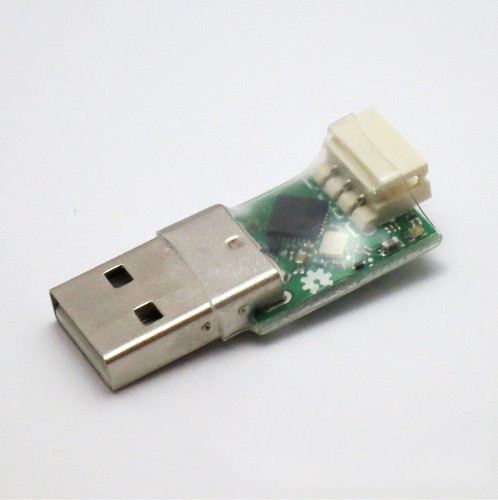
\includegraphics[height=5.5cm]{usb2ax.jpg}}
    \hfil
    \subfloat[][]{\label{fig:USB2AX_vs_USB2Dxl}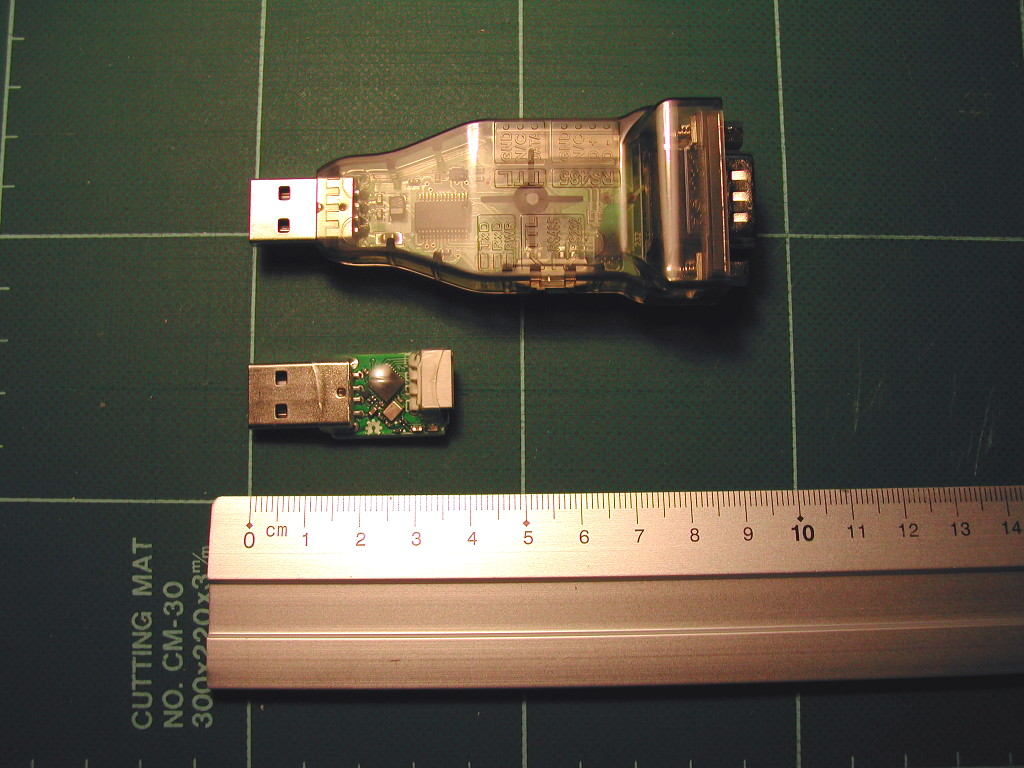
\includegraphics[height=5.5cm]{USB2AX_vs_USB2Dxl.jpg}}\\
    \caption{}
    \label{fig:usb2ax}
\end{figure}

\subsubsection{Arduino integration} % (fold)
The Arduino Due is a microcontroller board based on the Atmel SAM3X8E ARM Cortex-M3 CPU. It is the first Arduino board based on a 32-bit ARM core microcontroller. It has 54 digital input/output pins (of which 12 can be used as PWM outputs), 12 analog inputs, 4 UARTs (hardware serial ports), a 84 MHz clock, an USB OTG capable connection, 2 DAC (digital to analog), 2 TWI, a power jack, an SPI header, a JTAG header, a reset button and an erase button.
The board contains everything needed to support the microcontroller; simply connect it to a computer with a micro-USB cable or power it with a AC-to-DC adapter or battery to get started. The Due is compatible with all Arduino shields that work at 3.3V and are compliant with the 1.0 Arduino pinout.

The Poppy electronic architecture is based on two custom board: one to ensure communication with all input/output and another one for

\begin{figure}[tb]
    \begin{center}
        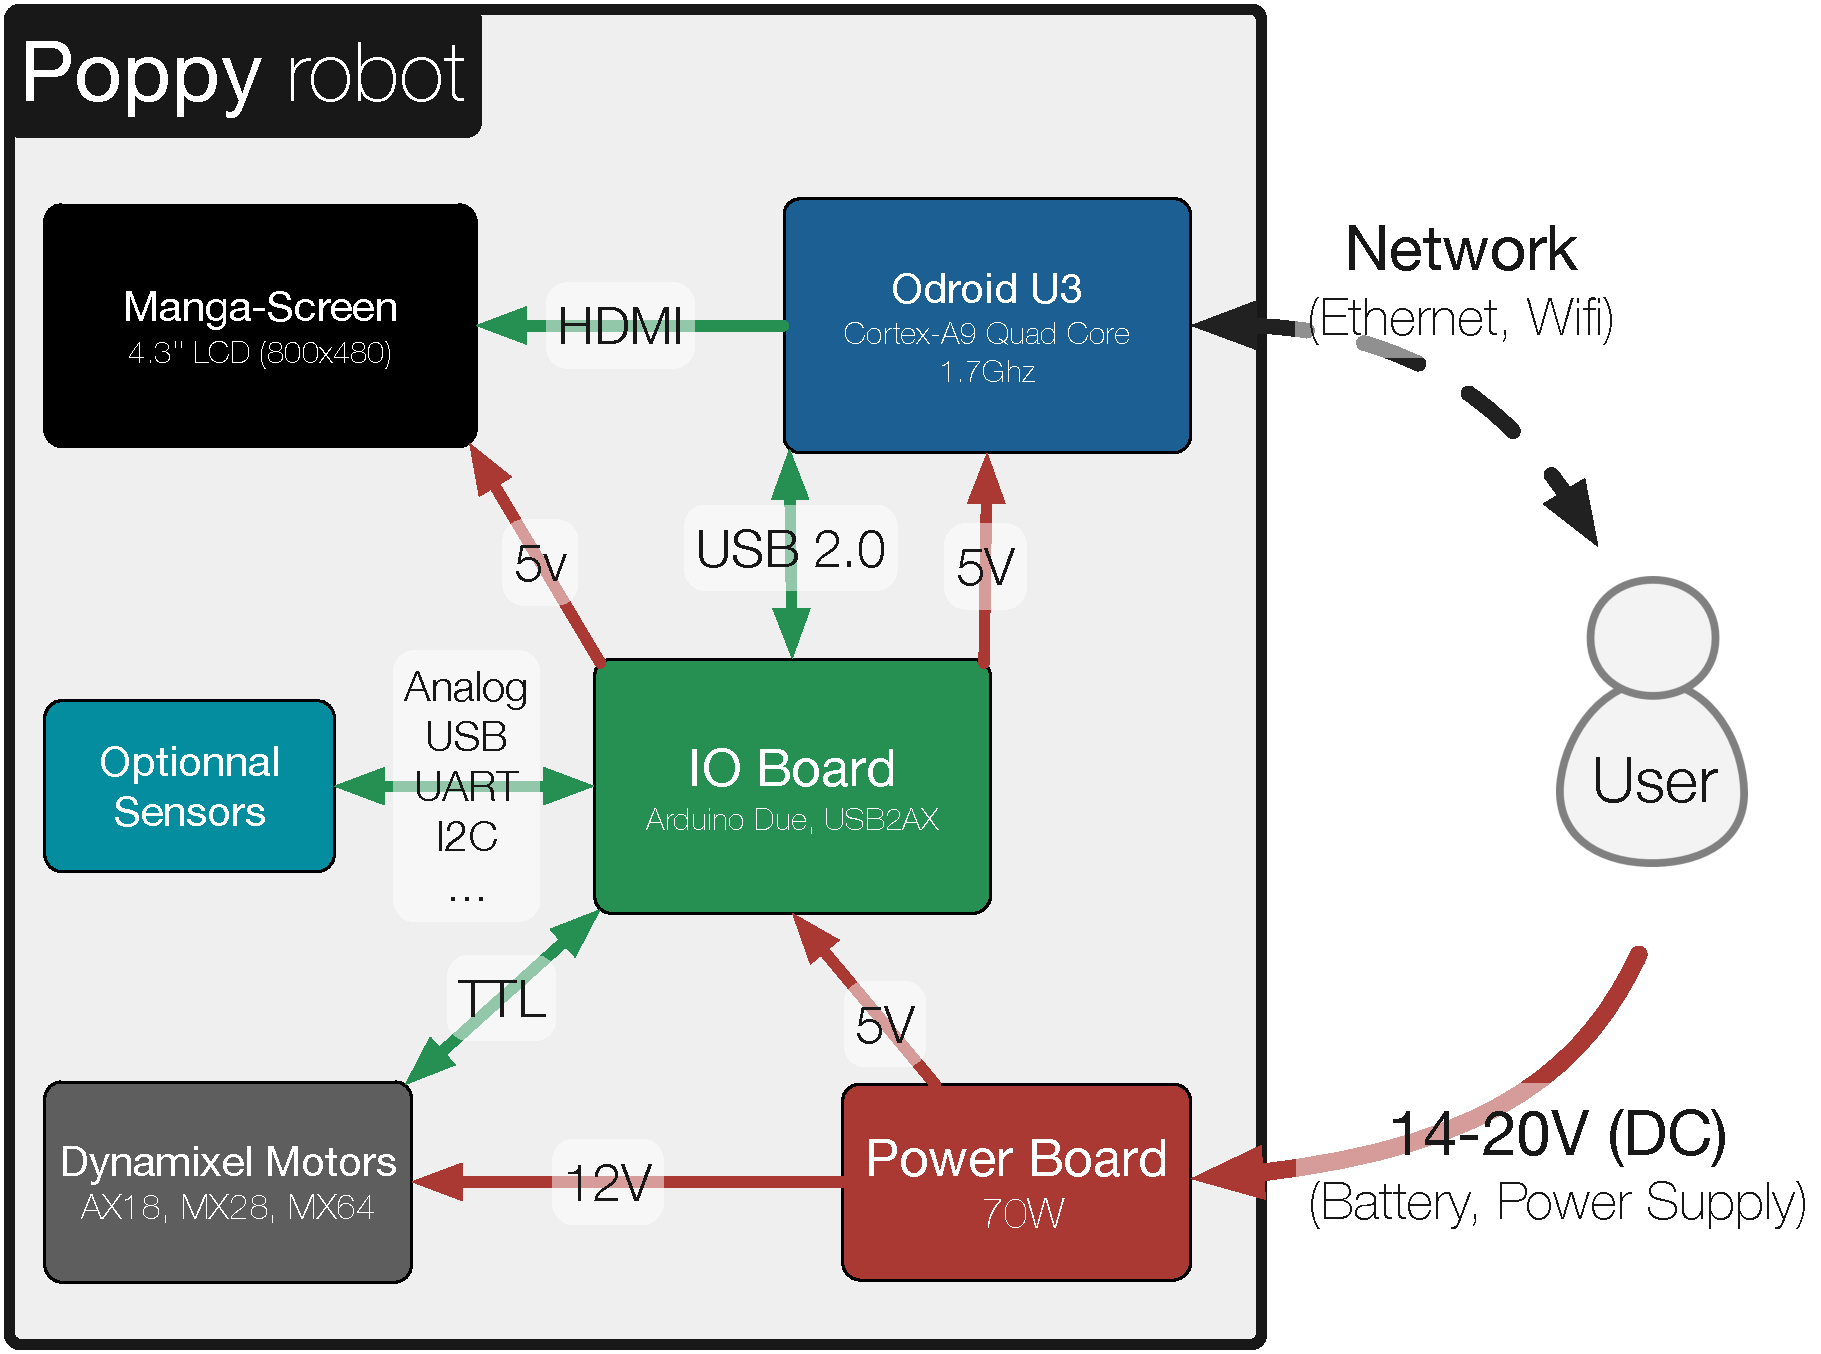
\includegraphics[width=\linewidth]{poppy_electro_archi_overview.pdf}
    \end{center}
    \caption{Caption here}
    \label{fig:figure1}
\end{figure}

\begin{description}
    \item[Computing:] Odroid U3
\end{description}


\subsection{Embedded computing module} % (fold)

The integration of a computing module is rather complex and not fundamental if the robot cannot walk for more than 5m, therefore the Poppy beta version was controlled using an external computer connected by USB.
However Poppy aims to become a shared research platform with people adressing challenge in which the embeded control can be necessary. Also as all user have a different computer configuration (Windows, MacOS and the plenty of Linux distribution), it is easier to maintain the control software if only one OS is used. Embedding a linux allows to have the control and ensure same performance for every Poppy.

Yet as I said previously, embedding control is complex. Indeed, the computer has to be small enough to fit inside the robot. With such size, where are mostly ARM based computer. Most of work are developed on x86 or 64 architecture and the switch to ARM architecture is not direct. Some software module used does not exist or are not optimized leading to big performance problems.

It is the case with one of the most famous micro-computer, the raspberry pi. The first trials we made using Pypot was really disappointing on the performance aspect. As we can see on the Figure Ref, it takes about 10-12 ms just to read and write a motor position (mostly computing) while it is only 2ms on a normal computer (mostly serial communication). Therefore we oriented our choice toward the Hardkernel Odroid U3 board (8\~12 times faster than the Raspberry Pi).

\begin{figure}[!h]
    \begin{center}
        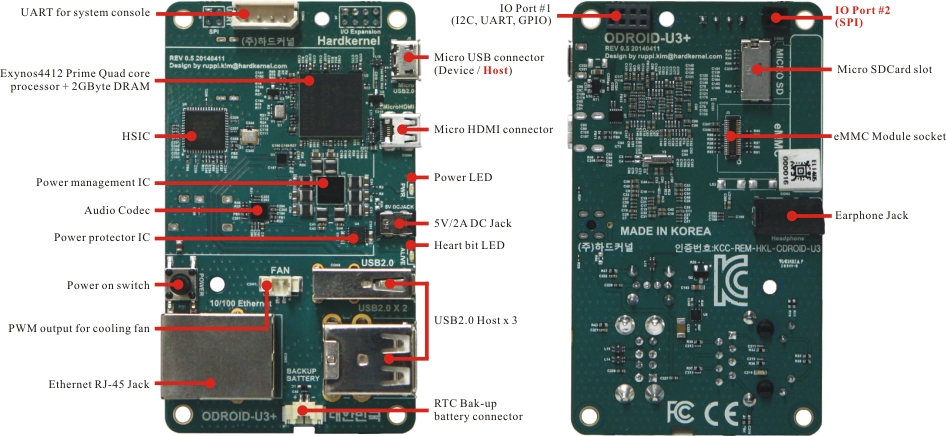
\includegraphics[width=\linewidth]{Odroid_U3.jpg}
    \end{center}
    \caption{Hardkernel Odroid U3 computer board}
    \label{fig:odroid_U3}
\end{figure}

The Hardkernel Odroid U3 (see \figurename~\ref{fig:odroid_U3}) is a low-cost (\$65) and powerful Linux computer embedding a 1.7GHz Quad-Core processor and 2GByte RAM while being very small (83 x 48 mm) and lightweight (48 grams) (see Tab.~\ref{tab:table_feet} for the detail of all specifications).

\begin{table}[!t]
    \begin{center}
        \begin{tabularx}{\linewidth}{r X}
        % \hline
        \textbf{Processor} & Samsung Exynos4412 Prime Cortex-A9 Quad Core 1.7Ghz with 1MB L2 cache\\
        \textbf{Memory} & 2048MB(2GB) LP-DDR2 880Mega data rate\\
        \textbf{3D Accelerator} & Mali-400 Quad Core 440MHz\\
        \textbf{Video} & supports 1080p via HDMI cable(H.264+AAC based MP4 container format)\\
        \textbf{Video Out} & micro HDMI connector\\
        \textbf{Audio} & Standard 3.5mm headphone jack HDMI Digital\\
        \textbf{LAN} & 10/100Mbps Ethernet with RJ-45 Jack ( Auto-MDIX support)\\
        \textbf{USB2.0 Host} & High speed standard A type connector x 3 ports\\
        \textbf{USB2.0 Device} & ADB/Mass storage(Micro USB), Host mode is possible if the PCB Rev is 0.5 or higher.\\
        \textbf{Display} & HDMI monitor\\
        \textbf{IO Port} & GPIO, UART, I2C, SPI(Board Revision 0.5 or higher)\\
        \textbf{Storage (Option)} & MicroSD Card Slot eMMC module socket\\
        \textbf{Power (Option)} & 5V 2A Power\\
        \textbf{System Software} & Linux : Xubuntu 13.10 or latest version Android : u-boot 2010.12, Kernel 3.0.x, Android 4.x  Full source code is available now.\\
        \textbf{PCB Size} & 83 x 48 mm\\
        \textbf{Weight} & 48g including the heat sink\\
         & \\
        % \hline
        \end{tabularx}
        \caption{Odroid U3 Linux computer detailed specifications}
        \label{tab:table_feet}
    \end{center}
\end{table}

Among the plug-n-play small computers, the Odroid U3 is currently the most suitable board for our application according to the size, the computing power and the I/O positions.
Yet as we will explain in the limitations (see section REF), this solution is still not perfectly satisfying and the use of plug'n'play computer raises a lot of integration problem.

\subsection{Display} % (fold)

The video out port on all new mini computer boards such as Raspberry Pi, Beagle board or Odroid boards is HDMI port. Finding small screen (< 7inch) compatible with HDMI input is really hard and currently only one project exists.The manga-screen (see \figurename~\ref{fig:manga-screen}) is a open source (CC-BY-SA\footnote{see REF}) multi purpose, HDMI compatible LCD screen. This board is developed by Elias Bakken and works with a 4.3 inch screen (480x800px) made by Sharp\footnote{Sharp LQ043Y1DX07}.

\begin{figure}[h]
\centering
    \subfloat[][]{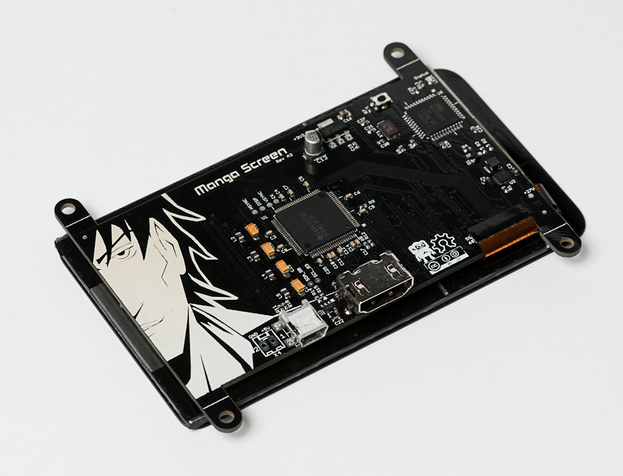
\includegraphics[height=4.9cm]{manga-screen.png}}
    \hfil
    \subfloat[][]{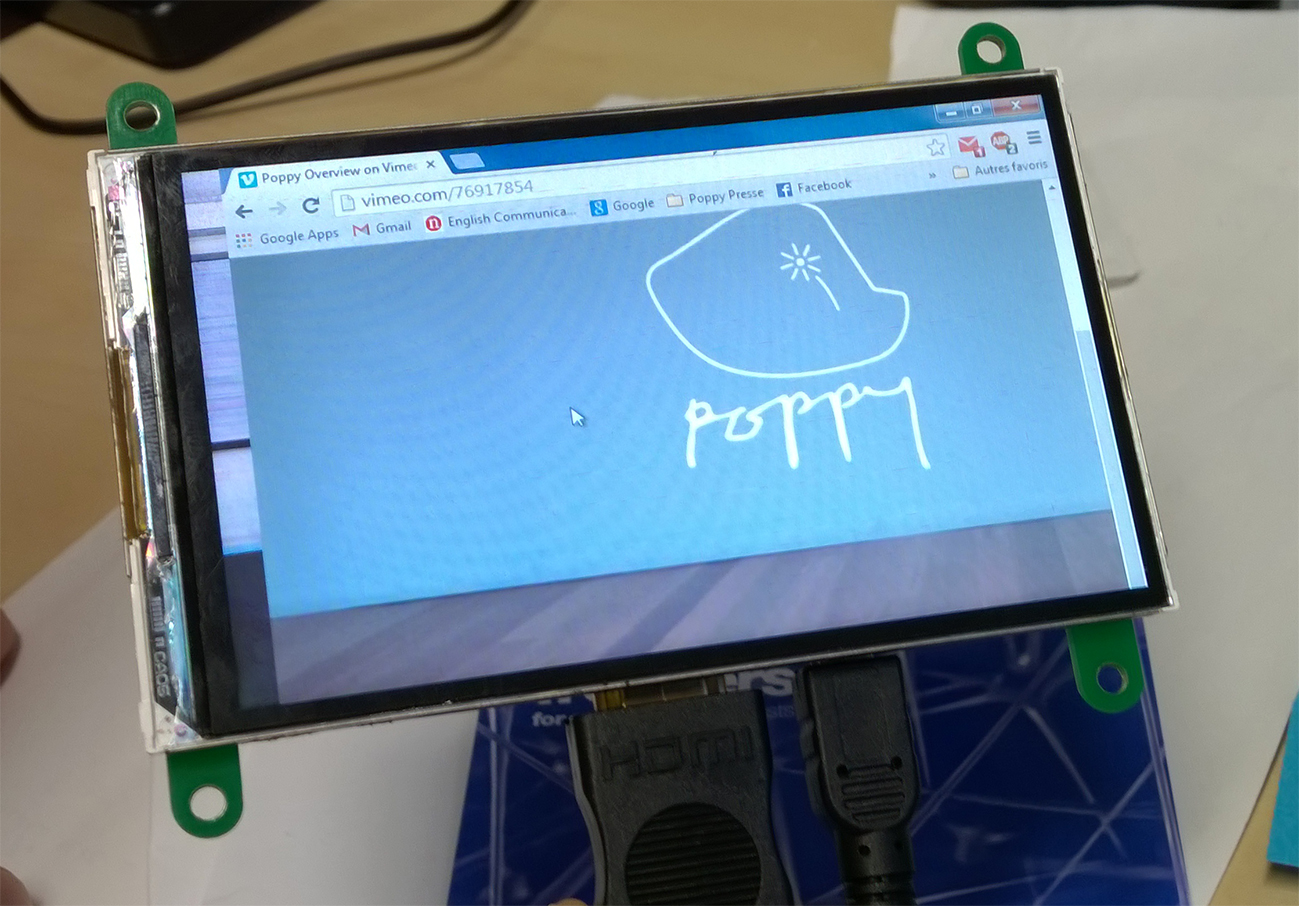
\includegraphics[height=4.9cm]{poppy_screen.jpg}}
    \caption{}
    \label{fig:manga-screen}
\end{figure}

The integration of a led matrix panel would be easier but it would require to create driver for the display.
Using a HDMI display connected to a Linux computer allows user to easily display information or animation on the screen like if it was on their monitor. Therefore they are free to use any tools they like such as Processing, OpenGL, VLC or whatever. This flexibility would not be possible with a matrix led panel which could basically only be used by Arduino.

% 56.16 × 93.60 mm active area R,G,B vertical stripes pixel configuration Black display mode 0.117 x 0.117 mm pixel pitch Mass 30 g

\subsection{IO Board} % (fold)

Most of the Poppy eletronical architecture is based on open source hardware projects. First,
\begin{figure}[]
\centering
    \subfloat[][]{\includegraphics[width=\linewidth]{IO_Board.pdf}}\\
    \subfloat[][]{\includegraphics[width=\linewidth]{IO_Board_mapping.png}}
    \caption{}
    \label{fig:}
\end{figure}

\begin{figure}[tb]
    \begin{center}
        \includegraphics[width=0.8\linewidth]{IO_board_simplify.jpg}
    \end{center}
    \caption{Caption here}
    \label{fig:figure1}
\end{figure}




\subsection{The battery issue} % (fold)
In the current design electronic architecture we did not include a battery. The main reason is the fact Poppy is not yet able to walk by itself so being energetically autonomous is not a high-priority.

Another issue associated with the batteries is the mass. A 3.6V battery cell weights around 45 grams and we need at least 4 cells to supply the 12V needed for Poppy, a 14,4V pack weights almost 200 grams (see \figurename~\ref{fig:battery_specs}). For comparison a MX-28 Dynamixels weights 72grams so with a battery weigths approximately the same mass as 3 motors.

Finally the overall size of such cell is rather big with 18mm x 65mm (see \figurename~\ref{fig:battery_size})

\begin{figure}[]
\centering
    \subfloat[][]{\label{fig:battery_size}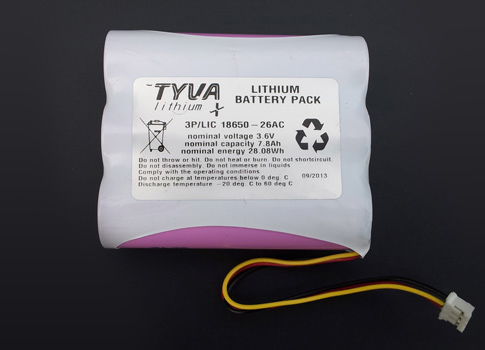
\includegraphics[height=3.5cm]{tyva_battery_pack.jpg}}
    \hfil
    \subfloat[][]{\label{fig:battery_specs}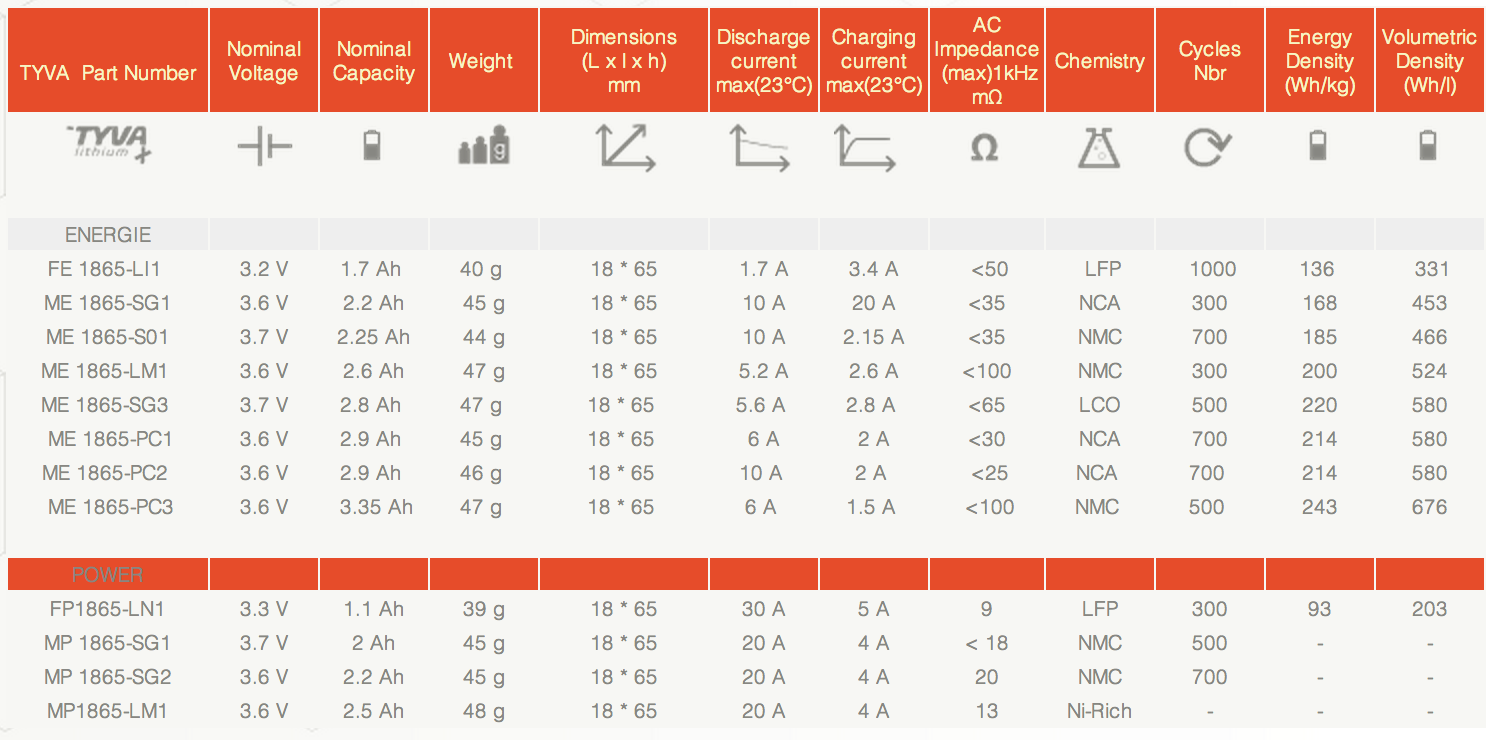
\includegraphics[height=4cm]{tyva_batteries.png}}\\
    \caption{}
    \label{fig:tyva_batteries}
\end{figure}





\subsection{Limitation} % (fold)

The electronic we developed is compatible with the exploration of morphology for sensory space because it has a lot of I/O ports to extend Poppy's sensorimotor space. Yet it has several limitations which make the final solution unsatisfying.

Commonly used electronic components are not designed for robotic integration but rather for building small personal computers. Thus even if the electronic boards are often quite smalls, they have big common connectors such as USB, HDMI, Ethernet which are of course never placed exactly where it should be for the integration in the robot.
Above all, cable are really annoying, they take surprisingly a lot of room (connector size, the wire length and they are heavy) while being totally useless for our applications.

Also the size of the IO Board is finally pretty big, more than expected and while it is still compatible with the Poppy design, it is too big with a too weird shape to be relevant for other open source project.

Great open source projects keep their work modular so other project can use directly one or several modules. Therefore the IO Board is not compatible with such principle and is currently under evolution toward the building of a modular Poppy electronics (we will discuss this new version in the discussion see REF). Yet this IO Board was the first electronic board developed in the Poppy project and the experience we acquire a better understanding of electronic integration. If we have to do it today we would make the same mistakes.

In particular, even if we tried to remove most of the necessary cables, we saw it is still complicated to make integration. We really have to develop board which do not require any wire at all.

Actually, I spent more time looking for the fitting cable on the web than thinking about the electronical architecture. The wire-problem is often under-estimated and therefore begin one the biggest problem for robotic. We experienced the same issue during the ergo-robot experiment and during the use of Poppy with artists (see chapter REF). SO basically, the wire problem is one of the most underrated issue.





\section{Hacking Poppy} % (fold)

\begin{figure}[tb]
    \begin{center}
        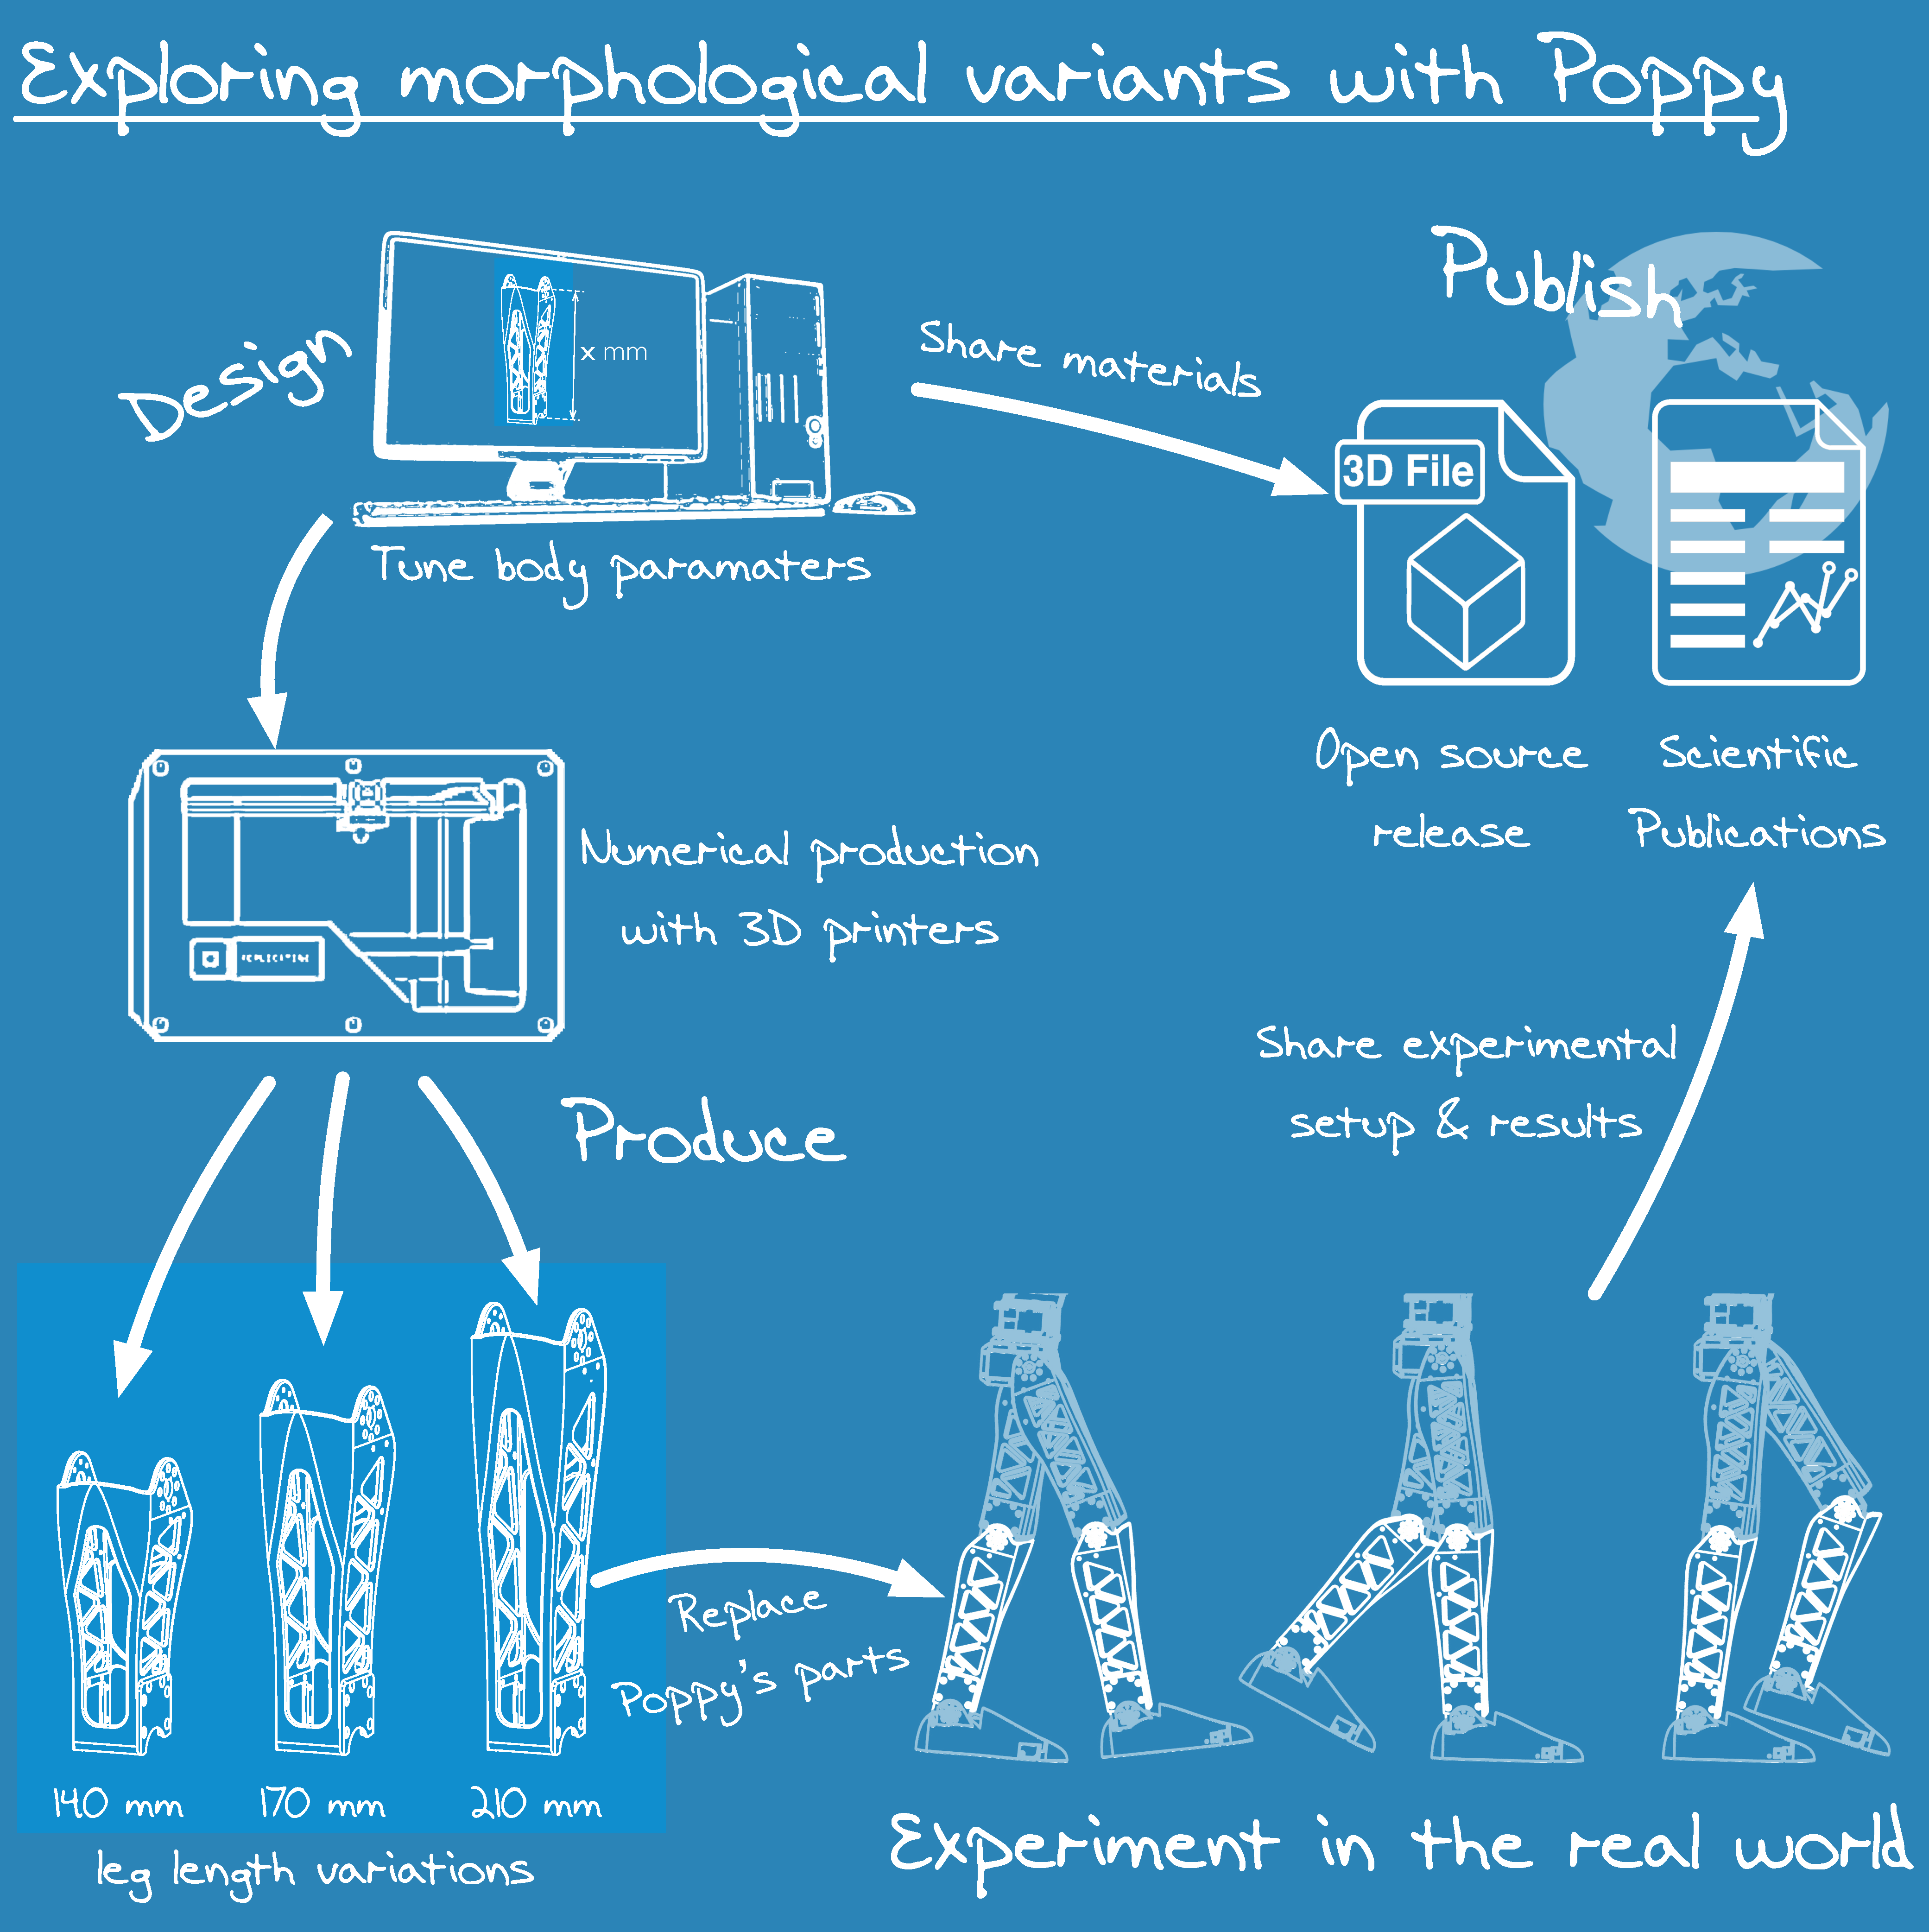
\includegraphics[width=\linewidth]{morpho_variation.pdf}
    \end{center}
    \caption{Caption here}
    \label{fig:figure1}
\end{figure}


\section{Discussion}

\section{Conclusion}

